\documentclass[11pt,a4paper]{article}

\usepackage[hyperref]{acl2017}
\usepackage{times}
\usepackage{latexsym}
\usepackage{graphicx}
\usepackage{subfigure}
\usepackage{amssymb}
\usepackage{amsmath}
\usepackage{bm}

\usepackage{xcolor}
\newcommand{\todo}[1]{\textcolor{red}{TODO: #1}\PackageWarning{TODO:}{#1!}}

\usepackage{url}

%\aclfinalcopy % Uncomment this line for the final submission
%\def\aclpaperid{***} %  Enter the acl Paper ID here

%\setlength\titlebox{5cm}
% You can expand the titlebox if you need extra space
% to show all the authors. Please do not make the titlebox
% smaller than 5cm (the original size); we will check this
% in the camera-ready version and ask you to change it back.

\newcommand\BibTeX{B{\sc ib}\TeX}



\title{Learning with Noise: Enhance Distantly Supervised Relation Extraction with Dynamic Transition Matrix\vspace{-10mm}}


\author{Bingfeng Luo, Yansong Feng, Zheng Wang, Zhanxing Zhu, \&
\and
Songfang Huang, Rui Yan \and Dongyan Zhao \\
  Institute of Computer Science \& Technology, Peking University, Beijing, China \\
  School of Computing and Communications, Lancaster University, Bailrigg, UK \\
  IBM China Research Lab, Beijing, China \\
  {\tt \{bf\_luo,fengyansong,zhanxing.zhu,ruiyan,zhaody\}@pku.edu.cn} \\
  {\tt z.wang@lancaster.ac.uk} \\
  {\tt huangsf@cn.ibm.com} \\}
  \author{Bingfeng Luo, Yansong Feng, Zheng Wang, Zhanxing Zhu, 
Songfang Huang, Rui Yan \and Dongyan Zhao \\
  Institute of Computer Science \& Technology, Peking University, Beijing, China \\
  School of Computing and Communications, Lancaster University, Bailrigg, UK \\
  IBM China Research Lab, Beijing, China \\
  {\tt \{bf\_luo,fengyansong,zhanxing.zhu,ruiyan,zhaody\}@pku.edu.cn} \\
  {\tt z.wang@lancaster.ac.uk} \\
  {\tt huangsf@cn.ibm.com} \\}

  



\begin{document}
\maketitle

\begin{abstract}
Distant supervision significantly reduces human efforts in constructing training data for many classification tasks, however, it inevitably introduces noise into the dataset. In this paper, we take a deep look at the application of distant supervision in relation extraction. We investigate the underlying noise in the training data, and propose to utilize constrained dynamic transition matrices to model the noise. We also take the advantage of curriculum learning to explore possible clues of the noise patterns, and further improve the model robustness. We experiment our models with both sentence level and bag level in the situations with and without prior knowledge of data quality. The experimental results show that our method can better handle the noise in distantly supervised relation extraction and improve extraction performance in various settings.

\end{abstract}
\section{Introduction}

\todo{ZW: Start by saying DS is a promoising technique for performing relation extraction on a large text corpus where manually labeling every single sentence is impossible. (2) The output of DS could be inherently noisy and low-quality data can significantly affect the results of relation extraction. 
     (3)There have been attempts on modelling/reducing the noise of DS, but prior work are terrible... (4) We then move to talk about our key insights,  how fantastic our approach is and how does it go beyond the state-of-the-art. (5) Summarise our experimental results, saying that we beat the state-of-the-art by xx\%.}

%Distant supervision is a commonly used method to automatically generate noisy training data with human designed heuristics. This method has been employed in many tasks including sentiment classification \cite{go2009twitter}, named entity recognition \cite{ritter2011named} and relation extraction \cite{mintz2009distant}. However,

%Sometimes, the heuristic only consists of a simple rule. For example, \cite{read2005using} considers the smile emoticon and the frown emoticon to expression positive and negative sentiment respectively and build a sentiment classification dataset with this heuristic. Sometimes, the heuristic depends on an existing database. For example,

Distant supervision is a way of exploiting existing (prior) knowledge to construct training data for classification tasks, without relying on laborious human annotation.

The basic distant supervision paradigm lies in making proper assumptions according to a task, distilling feasible and effective rules from prior knowledge and applying those rules to automatically prepare training data. Successful distant supervision applications include, relation extraction \cite{mintz2009distant}, cross-lingual semantic analysis \cite{fang2016learning}, and so on. The former assumes that the sentences containing both the subject and the object of a (subject $subj$, relation $rel$, object $obj$) triple are support for the existence of relation $rel$ between $subj$ and $obj$, and aligns triples in knowledge base with free text to automatically create training data. The latter assumes that words of different languages which share similar meaning should have similar POS tags, and thus automatically create training data for low-resourced languages according to their English translations.

%translates the English POS tag training data to other languages to compensate the the problem of limited training data for low-resourced languages.

Distant supervision significantly reduces the cost of obtaining training data for these tasks. However, since the assumptions may be imperfect, it also inevitably brings noise to the training data.  Sometimes the positive data may actually be negative (\emph{false positive}), while sometimes the negative data may actually be positive (\emph{false negative}). Furthermore, sometimes there may also be confusion between positive labels (\emph{positive label confusion}). This noisy data may disturb the training procedure, and lead to a model with inaccurate performance.

We need to note that, the noise introduced by distant supervision is not random, and the input data may consist of useful clues for us to identify its noise pattern. In relation extraction, for example, some sentences labeled by distant supervision to express the relation \emph{place\_of\_birth} between a person and place actually only talks about the work place of the person. Since we also find many sentences labeled as \emph{place\_lived} talks about the person's work place, we can reasonably assume that if a sentence is talking about the work place of a person, although the real relation expressed by the sentence is \emph{place\_lived}, there is still some chance that it is erroneously labeled as \emph{place\_of\_birth} by distant supervision.

This observation shows that it is possible to identify the noise pattern by analyzing the input data. In this paper, we propose to dynamically produce a transition matrix $\mathbf{T}$ for each datum to model the transition from the true label to the observed label. Here $T_{ij}$ represents the conditional probability that the observed label is $j$ given the true label is $i$. Since the label modeled by the transition matrix can be both positive and negative, it actually has the ability to model all the three types of noise introduced by distant supervision.

%The difficulty of training the transition matrix lies in that the only supervision we can use is the noisy label of the data.

%To overcome the difficulty, we propose to combine curriculum learning and trace normalization over the transition matrix to train our model.

In this paper, we focus specifically on the relation extraction task. The data is noisy because not all sentences containing $subj$ and $obj$ support the ($subj$, $rel$, $obj$) triple. \todo{for example...} In previous literature, this noise is often implicitly handled by the \emph{at-least-one assumption} that at least one of the sentences containing both $subj$ and $obj$ support the ($subj$, $rel$, $obj$) triple. The  sentences that containing both $subj$ and $obj$ are therefore aggregated into a sentence bag, and the problem becomes classifying the relation expressed by the sentence bag instead \cite{riedel2010modeling,lin2016neural}.


%Since the dataset proposed by \cite{luo2016temporal}, which aims at extracting relations between entity and time, contains both reliable and unreliable data, we also experiment our transition matrix model in the situation with and without reliable data.

However, the at-least-one assumption is not perfect either, and therefore introduces bag level noise. First, if all the retrieved sentences do not support the ($subj$, $rel$, $obj$) triple, then this bag is false positive. Second, if the ($subj$, $rel$, $obj$) triple is true but is missing in the KB, then the bag is false negative.
%Many methods have been developed to deal with this problem \cite{min2013distant,ritter2013modeling,xu2013filling}.

We apply our transition matrix method to both sentence level and bag level models. We also propose to combine curriculum learning and trace normalization for training to deal with the lack of guidance over the noise. The experiments show that our transition matrix method improve both of these models in two datasets. By experimenting on the dataset proposed by \cite{luo2016temporal}, which contains both reliable and unreliable data, we show that our training procedure can make use of the prior knowledge of the data quality and help the transition matrix model the noise better. We find that, the at-least-one assumption works better than the sentence level transition matrix model if no prior knowledge of the data quality is used. However, if we know which data are reliable, the sentence level transition matrix model works significantly better than bag level transition models. This shows that, with some indirect guidance, explicitly modeling the noise works better than using heuristics to implicitly handle the noise.

% In this paper, we propose to use transition matrix to model these noises in a unified form. Specifically, we want to dynamically generate a transition matrix $\mathbf{T}$ for each datum to model the transition from the real relation to the noisy relation tagged by distant supervision. Here $T_{ij}$ represents the conditional probability that the true relation of this sentence (or sentence bag) is $j$ given the relation assigned by distant supervision is $i$. By applying the transition matrix to sentence level models, our method can model the noise rather than just trying to lower the influcence of noisy data as previous methods do using \emph{at-least-one assumption}. Therefore, our method has the potential to actually make use of the noise rather than just trying to get rid of them. If our transition matrix is applied to bag level models, it can model both the false negative and false positive noise. Different from previous bag level denoising models, our models works in the neural network framework rather than the probabilistic graphic model framework. \todo{polish the difference from false negative models}

% We experiment our transition matrix method with both sentence level models and bag level models in two public relation extraction datasets. The experiments show that our transition matrix method can improve the performance of all baseline models in both datasets. We also find that, if we do not have prior knowledge of the data quality, the bag level model performs better than the sentence level model. However, if we have both reliable and unreliable data, we can use this prior knowledge to further improve the transition matrix. Since the sentence level noise is more important than the bag level noise, the sentence level model outperforms the bag level model in this situation, which shows that modeling the noise works better than just trying to ignoring the noise.

\section{Problem Definition}
The task of distantly supervised relation extraction is to extract knowledge tuples, i.e.,$<$\emph{subj},\emph{rel},\emph{obj}$>$, from free text using existing knowledge base, which can be applied in both the sentence and the bag
levels.  The former  takes a sentence $s$ containing both $subj$ and $obj$ as input, and outputs the relation expressed
by the sentence between $subj$ and $obj$. The latter setting is based on the \textit{at-least-one} assumption
 and takes a bag of sentences $S$ as input where each sentence
$s\in S$ contains both $subj$ and
$obj$, and output  the relation between $subj$ and $obj$ expressed by this bag.


This work aims to improve the state of the art in \DS for relation extraction.
We do so by first modeling the noise in the \DS generated training data using a dynamic transition matrix,  at both the sentence and the bag levels (Section~\ref{sec:approach}),  and then introducing a curriculum learning framework  to control the behavior of noise  under various training situations (Section~\ref{sec:training}).
%\red{Our model is applied at both the sentence and the bag levels. We evaluate approach
%in scenarios with and without prior knowledge of the data quality (Section xx).  we do not need the last sentence, right??}

%\todo{How to split data sets should go to experimental setup}


%In this paper, we will \orange{apply (changed from inject)} our noise modeling approach in both settings, and further investigate the performance of our approach in the situation with and without prior knowledge of the data quality. Specifically, we assume the prior knowledge can help us roughly distinguish reliable data from unreliable ones, and therefore split the dataset into several subsets with different levels of reliability. If no prior knowledge can be used, all the data are treated equally.


%In this paper, we apply transition matrix to two types of models. First, sentence level models take a sentence $s$ containing both $subj$ and $obj$ as input. We need to identify the relation expressed by the sentence between $subj$ and $obj$. Second, bag level models are based on the at-least-one assumption and take a bag of sentences $S$ as input where each sentence $s\in S$ contains both $subj$ and $obj$. We need to identify the relation expressed by the sentence bag between $subj$ and $obj$.

%\blue{DS is a powerful technique for performing relation extraction on a large text corpus where manually labeling every single sentence is impossible}
%
%Distantly supervised relation extraction aims at extracting $<$ $subj$,  $rel$,  $obj$ $>$ triples from free text using distantly obtained training data, which can be examined in two different settings, i.e., sentence level, and bag level. The former  takes a sentence $s$ containing both $subj$ and $obj$ as input, and output the relation expressed by the sentence between $subj$ and $obj$. The latter setting is based on the \textit{at-least-one} assumption (\todo{explain the assumption if not explained before}) and takes a bag of sentences $S$ as input where each sentence $s\in S$ contains both $subj$ and $obj$, and output  the relation expressed by the sentence bag between $subj$ and $obj$.

%\section{Motivation}
\todo{ZW: We need a concrete example here to demonstrate what kind of noise can exist in the data and their impact on relation extraction. We then use this example to explain our approach.}
\blue{F: this could be put into the introduction, saying different types of noises in the data, and all thoses noises can be modeled by TM. }

As a motivation example, consider xx...

This example shows that noisy data can have a significant impact on relation extraction. What we like to have is a technique that can xxx.
In the remainder of this paper, we describe such an approach based on xxx. 

%we experiment with the dataset proposed by \cite{luo2016temporal} which aims at extracting relations between entity and time. With some heuristics, this dataset can be further split intro three subsets with different levels of reliability, which enables us to conduct all our experiment settings. To show the generalization ability of our model, we also experiment with the dataset proposed by \cite{riedel2010modeling}, which aims at extracting relations between entities and there is no prior knowledge of the data quality can be used. \todo{can be shorter}

%We also consider two types of relation extraction tasks. The first task aims at extracting relations between entity and time. Specifically, it requires the object to be an time expression and the subject to be an entity. As suggested by \cite{luo2016temporal}, the distant supervision dataset in this task can be naturally divided into several subsets with different levels of reliability. The basic idea is that number of important things related to one entity increases as the time scope becomes larger. For example, a sentence containing both \emph{Alphabet} and \emph{October\_2\_2015} is very likely to express the foundation time of \emph{Alphabet}, while a sentence containing both \emph{Alphabet} and \emph{2015} may instead talk about its financial report of year 2015. We experiment with this task because it has a public dataset that contains both reliable and unreliable data, which enables us to conduct all of our experiments.

%The second task aims at extracting relations between entities, which is extensively studied in relation extraction. We experiment with this task to see if our transition matrix method generalizes well in different datasets.

\begin{figure}[t!]
\begin{center}
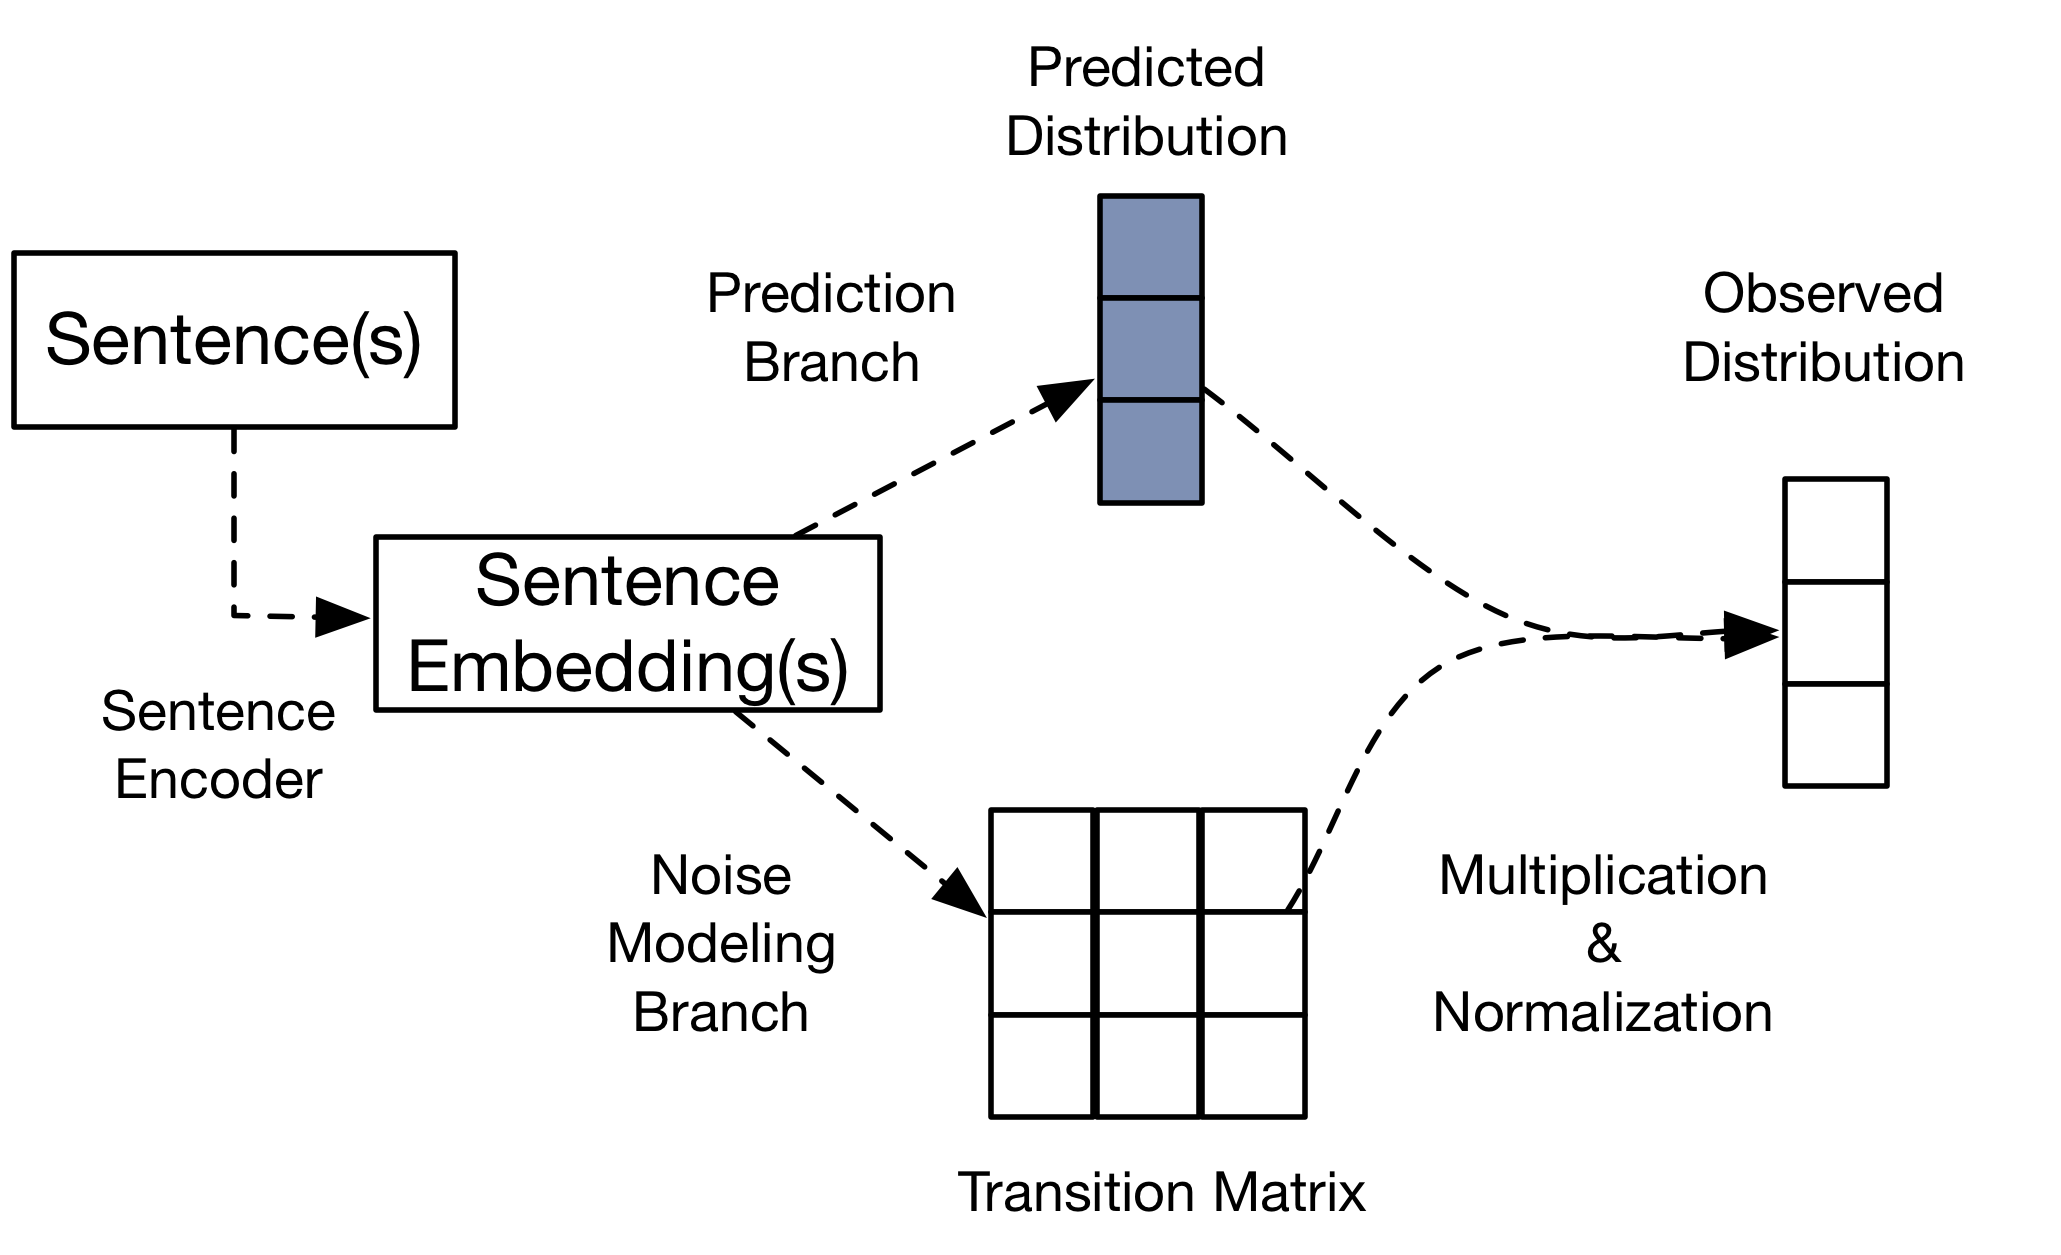
\includegraphics[width=8cm]{figures/denoise_framework.png}	
\caption{Overview of our approach}
\label{fig: denoise_framework}
\end{center}
\end{figure}


\section{Our Approach}
An overview of our approach of distantly supervised relation extraction is depicted in Figure \ref{fig: denoise_framework}. 
First, the input sentence (or sentence
bag) is passed to a sentence encoder to get sentence embedding(s). After that, the model is split into two branches.
The prediction branch generates the predicted relation distribution $\mathbf{p}$ of the input sentence (or sentence
bag). The noise modeling branch generates the transition matrix $\mathbf{T}$. Finally, the predicted distribution is
multiplied by the transition distribution to generate the observed relation distribution $\mathbf{o}$. The predicted
relation distribution $\mathbf{p}$ is the output of the model while the observed relation distribution $\mathbf{o}$ is
used to simulate the relation assigned by distant supervision. In this way, the noise is modeled by the transition
matrix and the real
prediction is protected from the influence of the noise. In rest of this section, we will first describe the sentence level model, and then extend the model to bag level.

\subsection{Sentence Encoder}
The sentence encoder serves to transform an input sentence to an embedding vector that encodes semantic meaning of the sentence. Theoretically, almost any sentence encoder would work here. Similar to previous researches, we also use the piecewise convolutional neural network (PCNN) model \cite{zeng2015distant} as our sentence encoder. First, the distances of each word to the subject and the object are embedded as randomly initialized vectors and concatenated to the original word vector. After that, the PCNN model divides the input sentence into three pieces by the subject and the object, and apply convolutional neural network (CNN) to each piece to calculate the piece embedding. The final sentence embedding is the concatenation of the embeddings of the three pieces.

\subsection{Prediction Branch}
The prediction branch generates the predicted relation distribution $\mathbf{p}$ and can be implemented by the prediction part of almost any relation extraction neural network models. Similar to \cite{luo2016temporal}, for sentence level models, we first feed the sentence embedding to a full connection layer, and then use softmax for relation classification.

\subsection{Noise Modeling Branch}
The noise modeling branch calculates a transition matrix dynamically for each sentence (or sentence bag) to model its noise pattern.

For sentence level models, the sentence embedding $\mathbf{x}$ is passed to another full connection layer to obtain the sentence embedding $\mathbf{x}_n$ used specifically for noise modeling branch. The transition matrix $\mathbf{T}$ is calculated using softmax function :
\begin{equation}
T_{ij} = \frac{exp({\mathbf{w}_{ij}^T \mathbf{x}_n + b})}{\sum_{j=1}^{|\mathbb{C}|}{exp({\mathbf{w}_{ij}^T \mathbf{x}_n + b}})}
\end{equation}
where $T_{ij}$ is the conditional probability that this sentence is labeled as relation $j$ by distant supervision given $i$ as the true relation, $\mathbf{w}_{ij}$ is the weight vector for this situation, $b$ is a scalar bias and $|\mathbb{C}|$ is the number of relations. Note that the softmax function guarantees that each row of the transition matrix $\mathbf{T}$ sums to 1.

\subsection{Observed Relation Distribution}
The observed relation distribution $\mathbf{o}$ is calculated by multiplying transition matrix $T$ and the predicted relation distribution $p$:
 \begin{equation}
\mathbf{o} = \mathbf{T}^T \bm\cdot \mathbf{p}
\label{eq_transition}
 \end{equation}
 \iffalse
 \begin{equation}
 \label{norm_o}
 o_i = \frac{o_i}{\sum_i{o_i}}
 \end{equation}
 \fi
 where $\bm\cdot$ represents dot product and we normalizes the elements of $\mathbf{o}$ so that $\sum_i{o_i}=1$ afterwards.

Different from previous works that use the predicted relation distribution $\mathbf{p}$ to directly match the relation labeled by distant supervision. \orange{We instead use $\mathbf{o}$ to match the noisy label and still use $\mathbf{p}$ as output}. Note that if the true relation of the input training instance is $i$, we can assume that this relation $i$ could be labeled as relation $j$ by distant supervision with probability $T_{ij}$. Therefore, Equation \ref{eq_transition} actually models the procedure of how the noisy label is produced and thus \orange{protects $\mathbf{p}$ from the bad influence of noise.}
%can help the model make better use of the noisy training data. \red{How to better use?? by using regularization????}

Also note that the noise modeling branch and $\mathbf{o}$ is only used in the training phase. In the test phase, we only use the prediction brach and take the predicted relation distribution $\mathbf{p}$ as our output. \todo{last paragraph can be removed}

\subsection{Bag Level Models}
\paragraph{Bag Level Prediction Branch}
The key problem in the bag level prediction branch is how to aggregate the embeddings of each sentence in the bag. Here we experiment with two methods, average and attention aggregation. The average aggregation calculates the bag embedding $\mathbf{s}$ by averaging the embeddings of each sentence, and the resultant bag embedding is fed to a softmax classifier for relation classification.

The attention aggregation method is proposed by \cite{lin2016neural}. It calculates an attention value for each sentence with respect to each relation, and uses the following equation to calculate the bag embedding with respect to relation $j$:
\begin{equation}
\mathbf{s}_j = \sum_i^{n}{\alpha_{ij} \mathbf{x}_{i}}
\label{eq_att_bag_embed}
\end{equation}
where $\mathbf{x}_{i}$ is the embedding of sentence $i$, $n$ is the number of sentences in the bag and $\alpha_{ij}$ is the attention value over sentence $i$ with respect to relation $j$. The resultant bag embedding is fed to a softmax classifier to predict the probability of relation $j$.

\paragraph{Bag Level Transition Matrix}
\orange{We use attention mechanism to generate transition matrix for both average and attention aggregation models.} Specifically, we calculate the bag embedding with respect to each relation with Equation \ref{eq_att_bag_embed}, and the attention value for sentence $i$ with respect to relation $j$ is calculated by:
\begin{equation}
\alpha_{ij} = \frac{exp(\mathbf{x}_i^T \mathbf{r}_t^j)}{\sum_i^n{exp(\mathbf{x}_i^T \mathbf{r}_t^j)}}
\end{equation}
where $\mathbf{x}_i$ is the embedding of sentence $i$ and $\mathbf{r}_t^j$ is the randomly initialized embedding of relation $j$ used specifically for noise modeling branch.

Then the transition matrix $\mathbf{T}$ is calculated by:
\begin{equation}
T_{ij} = \frac{exp({\mathbf{s}_i^T \mathbf{r}_t^j  + b})}{\sum_{j=1}^{|\mathbb{C}|}{exp(\mathbf{s}_i^T \mathbf{r}_t^j + b})}
\end{equation}
where $\mathbf{s}_i$ is the bag embedding with respect to relation $i$, $\mathbf{r}_t^j$ is the same embedding of relation $j$.


\section{Training Procedure}
\red{I would suggest to move some of the motivations to the Introduction part,  we need to motivate regularization and CL there.}The difficulty of training the transition matrix lies in that there is no direct guidance over the noise pattern. The only supervision we have is the noisy label produced by distant supervision. However, if we have prior knowledge to roughly separate the data into reliable and unreliable parts, we can use the split as indirect supervision over the noise pattern by letting the model treat these data differently. In this section, we describe how to use trace regularization to control the behavior of the transition matrix. Furthermore, instead of modeling the noise at the very beginning of the training, we emphasis noise modeling gradually by building different curriculums in the situation with and without prior knowledge of the data quality under the curriculum learning framework.
%Apart from that, we also show how to constrain the \red{ability??} of the transition matrix to avoid \red{overfitting???}.

\subsection{Trace Regularization}
Intuitively, if the noise is small, the transition matrix $\mathbf{T}$ will tend to become an identity matrix (vice versa).  Since each row of $\mathbf{T}$ sums to 1, the similarity between the transition matrix and the identity matrix can be represented by the trace of the transition matrix $\mathbf{T}$. The larger the $trace(\mathbf{T})$ is, the smaller the elements that do not lie in the diagonal are, and the more similar the transition matrix $\mathbf{T}$ is to identity matrix. Therefore, we can realize our expectation over the noise level of the data by controlling the value of $trace(\mathbf{T})$.

\subsection{Curriculum Learning}
The basic idea of curriculum learning is simple: start with the easiest aspect of a task, and level up the difficulty gradually.

\paragraph{With Prior Knowledge of Data Quality}
If we have prior knowledge about which part of the training data is more reliable and which is unreliable, the most straightforward way to build a curriculum is by controlling the reliability of training data. Specifically, we can first train the prediction branch on the reliable data for some epochs and then add the unreliable data \orange{to train the full model}. In this way, the prediction branch is roughly trained before exposed to more noisy data.

Furthermore, \orange{we can also take better control of the training procedure by trace regularization.}
%\red{utilize our prior knowledge of the data quality in the form of trace regularization}.
Specifically, our loss function is:

\begin{equation}
\begin{aligned}
Loss=\sum_{i=1}^M{\sum_{j=1}^{N_i}{-log(o_{ijy_{ij}})}} + \beta_i trace(\mathbf{T}_{ij})
\end{aligned}
\end{equation}
where the left side is vanilla cross entropy and the right side is trace regularization, $i$ is the index of the data subsets, $j$ is the index of training data, $\beta_i$ is the trace regularization weight for subset $i$, $\mathbf{T}_{ij}$, $y_{ij}$ and $o_{ijy_{ij}}$ are the transition matrix, relation labeled by distant supervision, and the observed probability of that relation for datum $j$ in subset $i$ respectively.

For the reliable subset, we want $trace(\mathbf{T})$ to be large (negative $\beta$) so that the element values of $\mathbf{T}$ will be centralized to the diagonal and the transition matrix will be similar to identity matrix. As for the unreliable subsets, we want the $trace(\mathbf{T})$ to be small (positive $\beta$) so that the element values of their transition matrices will be diffusive \orange{and the transition matrix will be less similar to identity matrix. In other words, the transition matrix is encouraged to model the noise}. Note that this loss function only works for sentence level models, since reliable sentences and unreliable ones are all aggregated into a sentence bag in the bag level models and therefore we can not determine which bag is reliable and which is not. However, bag level models can still use the curriculum by changing the content of the bag, \orange{and can therefore benefit from the prior knowledge of data quality.}

\paragraph{Without Prior Knowledge of Data Quality}
\label{curr_over_data}
If we do not have prior knowledge about the quality of training data, we can still build a curriculum, which can be used in all situations, \orange{by controlling the training objective to gradually emphasis on noise modeling. Specifically, we design a decreasing weighting scheme for both the cross entropy of output prediction and the trace regularization component: (CHANGE EXPLAINATION: the decreasing scheme is for both $\alpha$ and $\beta$, not just $\beta$.)}
%\red{ gradually controlling the impact of the transition matrix}. Specifically, \red{we design a decreasing weighting scheme for the trace regularization component}, defined as:

\begin{equation}
\begin{aligned}
Loss	&=\sum_{i=1}^N{-((1-\alpha) log(o_{iy_{i}}) + \alpha log(p_{iy_{i}}))} \\
&+ \beta trace(\mathbf{T}_{i})
\end{aligned}
\end{equation}
where $0\le\alpha\le1$, $y_i$ is the relation assigned by distant supervision for datum $i$, $o_{iy_{i}}$ and $p_{iy_{i}}$ are the probabilities that the observed and predicted relation for datum $i$ is $y_i$ respectively. Instead of only using the observed relation distribution $\mathbf{o}$ to simulate the relation labeled by distant supervision, we use the linear combination of the cross entropy of both the observed relation distribution $\mathbf{o}$ and the predicted relation distribution $\mathbf{p}$.

\orange{We consider ignoring the noise is easier than modeling the noise. Therefore, to build a curriculum}, we set $\alpha=1$ and $\beta<0$ at the start of the training, which means we do not expect to model the noise. As the training proceeds, the prediction branch gradually learns the basic prediction ability, then we increase the difficulty level by decreasing $\alpha$ and the absolute value of $\beta$ by $\rho$ every $\tau$ epochs to gradually guide our model to learn to model the noise.

\subsection{Constrained Transition Matrix}
\orange{Since the triples in knowledge base are reliable in most of the times, the positive label confusion noise is less likely than the false negative and false positive noise.} However our transition matrix has the ability to model all these three types of noise. To prevent overfitting and make the model \red{concentrate on the false negative and false positive noise??}\orange{(not sure about the problem)}, we restrict the transition matrix for bag level models so that only the diagonal, the first column and the first row of the transition matrix do not equal to zero (assume the index of \emph{no-relation} is 0).

\section{Curriculum Learning based Training \label{sec:training}}
%Training with Curriculum Learning??
%\blue{we talk about the difficulty of training with $\sum_{i=1}^N{-log(o_{iy_{i}}) } + \beta trace(\mathbf{T}_{i})$  first. 1) noisy data, 2) local optima. Therefore, we need CL. The advantages are 1) learn to model with noise gradually, 2) more robust, avoid local optima, 3) have a chance to control the effect of noise via Trace norm.  }

One of the key challenges of this work is  on how to train and produce the transition matrix to model the noise without any direct guidance and human involvement in the training data.
A straightforward solution is to directly align the observed distribution, $\mathbf{o}$, with respect to the noisy annotations by minimizing the sum of the two terms:
$CrossEntropy(\mathbf{o}) + Regularization$. However, doing so
does not guarantee that the prediction distribution, $\mathbf{p}$, will match the true relation distribution.
The problem is at the beginning of the training, we have no prior knowledge about the noise pattern; thus, both  $\mathbf{T}$ and $\mathbf{p}$ are less reliable, which will make the training procedure be likely to trap into some poor local optimum.
Therefore, what we would like to have is a technique to guide our model to gradually adapt to the noisy training data, e.g., learning something simple first, and then trying to deal with noises.

Fortunately, this is exactly what curriculum learning can do.
The idea of \red{curriculum learning~\cite{}} is simple: starting with the easiest aspect of a task, and leveling up the difficulty gradually,
which fits well to our problem.
We thus employ a curriculum
learning framework to guide our model to gradually learn how to characterize the noise. 
% and how to control its effect via trace regularization, while 
Another advantange is to avoid falling into poor local optimum,
when there is little knowledge about the noise pattern. 


By exploring curriculum learning, our approach  provides the
flexibility to combine any prior knowledge of noise to improve the
effectiveness of  the transition matrix. 
We show that if one could break the
dataset into reliable and less reliable parts, our approach can exploit the split
as indirect supervision over the noise pattern to build more effective
transition matrix to better model the noise. The sum is greater than its parts.
As shown later in Section~\ref{sec:evaluation}, putting together these techniques
enables us to build an adaptive scheme to better model the noise pattern over the state-of-the-art.



%Furthermore, if we have prior knowledge to roughly separate the data into reliable and less reliable subsets, we can utilize the split as indirect supervisions over the noise pattern to help the transition matrix to better model the noise.
%Apart from that, we also show how to constrain the \red{ability??} of the transition matrix to avoid \red{overfitting???}.

\subsection{Trace Regularization}
Before proceeding to training details, we first discuss how we characterize the noise level of the data by controling the trace of the transition matrix.
Intuitively, if the noise is small, the transition matrix $\mathbf{T}$ will tend to become an identity matrix, i.e., given a set of annotated training sentences,  the observed relations and their true relations are almost identical. Since each row of $\mathbf{T}$ sums to 1, the similarity between the transition matrix and the identity matrix can be represented by the trace of $\mathbf{T}$, $trace (\mathbf{T})$. The larger the $trace(\mathbf{T})$ is, the larger the diagonal elements are, and the more similar the transition matrix $\mathbf{T}$ is to the identity matrix, indicating a lower level of noise. Therefore, we can characterize  the noise level of the data by controlling the \sout{\red{expected}} value of $trace (\mathbf{T})$ in the form of regularization. For example, we will expect a larger $trace (\mathbf{T})$ for reliable data, but  a smaller $trace (\mathbf{T})$  for less reliable data. Another advantage of employing trace regularization is that it could be helpful to reduce the model complexity,  %since we have so many parameters (each data has a TM),
and avoid overfitting.

%\subsection{Curriculum Learning}
%The idea of curriculum learning is simple: starting with the easiest aspect of a task, and leveling up the difficulty gradually, which fits well with our problem.
%There are situations where we may have prior knowledge of the data quality and situations where we do not.
%Curriculum learning performs well in both scenarios.

\subsection{Training}
%\paragraph{Without Prior Knowledge of Data Quality}
To tackle the challenge of no direct guidance over the noise patterns,
%i.e., $\mathbf{p}$ does not guarantee to match the true relation distribution,
we implement a curriculum learning based training method to
%a straightforward idea is to
first train the model without considerations for noise. In other words, we first focus on the loss from the prediction distribution $\mathbf{p}$ ,  and then take the noise modeling into account gradually along the training process, i.e., gradually increasing the importance of the loss from the observed distribution $\mathbf{o}$ while decreasing the importance of $\mathbf{p}$. In this way, the prediction branch is roughly trained before the model managing to characterize the noise, thus avoids being stuck into local optimum.
%We implement this idea in the curriculum learning framework, and,  specifically,
%we consider ignoring the noise is the easier part of training compared with modeling the noise, and our
We accordingly design to minimize  the following loss function:
%
%If no guidance over the noise pattern exists, using only $\mathbf{o}$ to match the noisy label does not guarantee $\mathbf{p}$ to match the true relation distribution. Therefore, we use the linear combination of the cross entropy of both $\mathbf{o}$ and $\mathbf{p}$ as our objective function. Furthermore, we build a curriculum by controlling the training objective to gradually emphasis on noise modeling. Specifically, we design a decreasing weighting scheme for both the cross entropy of output prediction and the trace regularization component:
%\red{ gradually controlling the impact of the transition matrix}. Specifically, \red{we design a decreasing weighting scheme for the trace regularization component}, defined as:
%
\begin{equation}
\begin{aligned}
Loss	&=\sum_{i=1}^N{-((1-\alpha) log(o_{iy_{i}}) + \alpha log(p_{iy_{i}}))} \\
&- \beta trace(\mathbf{T}^{i})
\end{aligned}
\label{general_loss}
\end{equation}
where $0>\alpha>1$ and $\beta>0$ are two weighting parameters, $y_i$ is the relation assigned by \DS for the $i$th training instance, $N$ the total number of training instances , $o_{iy_{i}}$ is the probability that the observed relation for the $i$th instance is $y_i$, and $p_{iy_{i}}$ is the probability that the predicted relation for the $i$th instance is $y_i$.
%and $p_{iy_{i}}$ are the probabilities that the observed and predicted relations for the $i$th instance are $y_i$ respectively.
%Instead of using the observed relation distribution $\mathbf{o}$ only to simulate the relation labeled by \DS, we use the linear combination of the cross entropy of both the observed relation distribution $\mathbf{o}$ and the predicted relation distribution $\mathbf{p}$. \blue{do we need a reason or two?}

Initially, we set $\alpha=1$, and train our model  completely by minimizing the loss from the prediction distribution $\mathbf{p}$. That is, we do not expect to model the noise,  but focusing  on the prediction branch at this time. As the training progresses, the prediction branch gradually learns the basic prediction ability. We then decrease $\alpha$ and  $\beta$ by $0<\rho<1$ \orange{($\alpha=\rho\alpha$ and $\beta=\rho\beta$)} every $\tau$ epochs i.e., learning more about the noise from the observed distribution $\mathbf{o}$ and allowing a relatively smaller $trace(\mathbf{T})$ to accommodate more noise.
% , to gradually shift part of our focus to \orange{noise modeling.} 
%\red{learning with noise}. 
The motivation behind is to put more and more effort on learning the noise pattern during training, 
with the essence of curriculum learning.
This gradually learning paradigm significantly distinguishes from prior work on noise modeling for \DS seen to date. 
Moreover, as such a method does not rely on any extra assumptions,
it can serve as our default training method for $\mathbf{T}$.

\paragraph{With Prior Knowledge of Data Quality}
On the other hand, if we happen to have prior knowledge about which part of the training data is more reliable and which is less reliable, we can utilize this knowledge as an indirect guidance over the noise patterns \red{by helping the model to distinguish reliable data from less reliable ones (DO WE actually distinguish them??)}\orange{yes, with trace reg, and indirectly with CL as well}. Specifically, we can build a curriculum by first training the prediction branch on the reliable data for several epochs, and then adding the less reliable data to train the full model. In this way, the prediction branch is roughly trained before exposed to more noisy data, thus is less likely to fall into poor local optimum.

Furthermore, we can take better control of the training procedure by using trace regularization, e.g., encouraging larger $trace (\mathbf{T})$ for reliable subset and smaller $trace (\mathbf{T})$ for less relaibale ones.
%\red{utilize our prior knowledge of the data quality in the form of trace regularization}.
Specifically, we propose to minimize the following  loss function:
%
\begin{equation}
\begin{aligned}
Loss=\sum_{m=1}^M{\sum_{i=1}^{N_m}{-log(o_{miy_{mi}})}} - \beta_m trace(\mathbf{T}^{mi})
\end{aligned}
\end{equation}
where $\beta_m$ is the regularization weight for the $m$th data subset, $N_m$ is the total number of instances in $m$th subset, and  $\mathbf{T}^{mi}$, $y_{mi}$ and $o_{miy_{mi}}$ are the transition matrix, the relation labeled by distant supervision and the observed probability for the $i$th training instance in the $m$th subset, respectively. Note that different from Equation~\ref{general_loss}, this loss function does not need to initiate the training procedure by
minimizing the loss regarding the prediction distribution $\mathbf{p}$, since one can easily start by learning from the most reliable split first. 
%since we have indirect guidance over noise pattern here. Specifically, trace regularization can utilize the prior konwledge of data quality by using different weights to serve as indirect guidance over noise pattern. Therefore,  
%\orange{change the reason to trace reg?}

For the reliable subset, we want $trace(\mathbf{T})$ to be large (positive $\beta$) so that the element values of $\mathbf{T}$ will be centralized to the diagonal and $trace (\mathbf{T})$ will be more similar to the identity matrix. As for the  less reliable subset, we want the $trace (\mathbf{T})$ to be small (negative $\beta$) so that the element values of their transition matrices will be diffusive and the transition matrix will be less similar to the identity matrix. In other words, the transition matrix is encouraged to characterize the noise.

It is to note that this loss function only works for sentence level models. Since reliable sentences and less reliable ones are all aggregated into a sentence bag in the bag level models,  we can not determine which bag is reliable and which is not. However, bag level models can still use the curriculum by changing the content of the bag, e.g., keeping reliable sentences in the bag first and gradually adding less reliable ones, and use Equation~\ref{general_loss} for training. By doing so, it can benefit from the prior knowledge of data quality as well.



%%%%%%%%%%%%%%%%%%%% omit for further journal publication  %%%%%%%%%%%%%%%%%%%%%%%%%%%%%%
%%
%%
%\subsection{Constrained Transition Matrix} \blue{DO we need special discussion for this one??}
%%%\orange{Since the triples in knowledge base are reliable in most of the times, the positive label confusion noise is less likely than the false negative and false positive noise.}
%\red{In most DS relation extraction cases,  the imperfect knowledge bases and the inexact alignments between seed knowledge facts and unstructured text lead to many  \textit{false negative} and \textit{false positive} instances, more severe compared to  the \textit{label confusions} issues among positive relations.
%%%the problems of \textit{false negative} and \textit{false positive} are more severe, compared to \textit{label confusions} among positive relations.
%%%The reasons are twofold. First, since the knowledge bases are usually far from perfect, the \DS generated negative data are often \textit{false negative}. And the inexact alignments between seed knowledge facts and unstructured text produces many  \textit{false positive} instances.
% }
%%%However our transition matrix has the ability to model all these three types of noise. To prevent overfitting and make the model \red{concentrate on the false negative and false positive noise??}\orange{(not sure about the problem)},
%We  thus restrict the transition matrix for bag level models to \blue{(why not sentence level?)} so that the diagonal, the first column and the first row of the transition matrix may not equal to zero\footnote{we assume that the index of \emph{No-Relation} is 0.}, \blue{acommodating  such noisy instances???}.
%%
%%
%%
%%%%%%%%%%%%%%%%%%%% omit for further journal publication  %%%%%%%%%%%%%%%%%%%%%%%%%%%%%%
%

\section{Evaluation}
\subsection{Data Sets}
We experiment our model on two datasets. The first one is proposed by \cite{luo2016temporal} and aims at extraction relations between entity and time (\emph{time RE data}). The dataset is constructed by aligning Wikidata triples with Wikipedia corpus. Based on the granularity of the time expression in the sentence, this dataset can be split into 3 subsets with different levels of reliability. The reliable subset is used as basic training data, validation data and test data which contains 22,214, 2,776 and 2,771 positive sentences respectively. The two less reliable subset contains 2,094 and 53,469 positive sentences and are used as additional training data. Negative data are constructed with two heuristic strategies. We use this dataset because this is a public dataset on relation extraction that has both reliable and unreliable data, which is suitable for all of our experiment settings.

We also conduct our experiment on the dataset proposed by \cite{riedel2010modeling}, which is a commonly used dataset in relation extraction (\emph{entity RE}). This dataset is generated by aligning triples in Freebase with the New York Times corpus (NYT corpus). The training data contains 522,611 sentences and 281,270 entity pairs. The test set contains 172,448 sentences and 96,678 entity pairs. We experiment our bag level models in this dataset to see the generalization ability of our transition matrix model.


\subsection{Hyper-parameters}
\paragraph{Sentence Level Model}
We experiment our sentence level model on time RE data. We use 100-dimensional word embedding pre-trained using GloVe \cite{pennington2014glove} on Wikipedia and Gigaword, and 20-dimensional vector for distance embedding. The convolution window is 3 and the number of convolution kernels is 200. The size of the full connection layer is also 200. As for training, we use stochastic gradient descend (SGD) for optimization with batch size 20, learning rate 0.1. We also use dropout with probability 0.5 upon the sentence embedding. Each phase of the curriculum learning over dataset contains 15 epochs. The trace normalization parameters for three subsets are $\beta_1=-0.01$, $\beta_2=0.01$ and $\beta_3=0.1$ (the ratio of $\beta_3$ and $\beta_2$ is fixed to 10 and 5 when tuning hyper-parameters).

\paragraph{Bag Level Model}
The parameters of the bag level model is almost the same as the sentence level model on time RE data, except that the learning rate is 0.01. As for entity RE data, our settings for prediction branch is similar to \cite{lin2016neural}. The word embedding is of dimension 50 and is pre-trained on the NYT corpus using word2vec\footnote{\url{ https://code.google.com/p/word2vec/}}. The convolution window is 3 and the number of convolution kernels is 256, distance embedding size is 5, batch size is 16 and learning rate is 0.01. For all the bag level models, the linear combination parameter $\alpha$ is 1 and trace normalization parameter $\beta$ is -0.1 at the start of training. We experiment with decay rate \{0.95, 0.9, 0.8\} and decay step \{3, 5, 8\}. We find that using decay rate 0.9 and decay step 5 performs well in most situations.

\begin{figure}[htbp]
\begin{center}
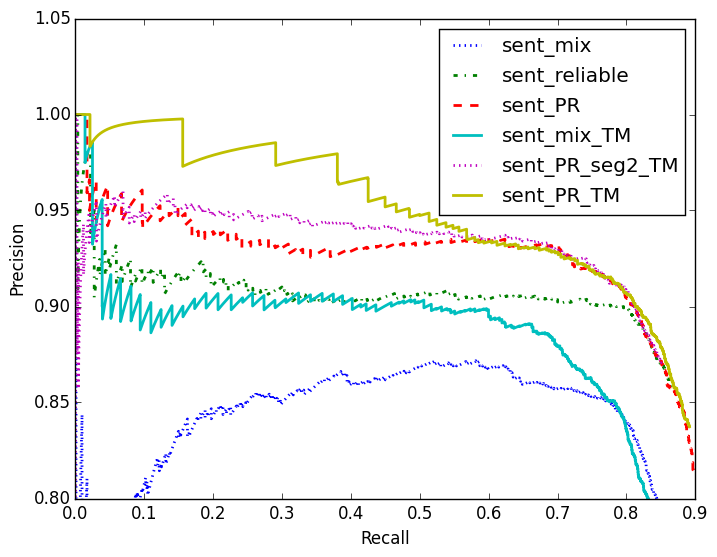
\includegraphics[width=0.9\linewidth]{figures/sent_time_exp_overall.png}
\caption{Sentence Level Results on Time RE}
\label{fig: sent_luo}
\end{center}
\end{figure}

\subsection{Results on Time RE Data}
We exhibit the results in the form of precision recall curves (PR curves).

\paragraph{Sentence Level Models}
The results of sentence level models is shown in Figure \ref{fig: sent_luo}. We can see that the performance of the model trained on all subsets mixed together (\emph{sent\_mix}) is very bad, which is significantly worse than the model trained only on the reliable subset (\emph{sent\_reliable}). This shows that the noise problem is innegligible and have bad influence on the training of the model. However, with the help of transition matrix, the model obtains the ability of modeling noise (\emph{sent\_mix\_TM}), which significantly improves the performance of the model. By using the reliable subset first and gradually adding less reliable data (\emph{sent\_curr}), we can see that the model can actually make use of the noisy data and performs better than the model trained only on the reliable subset. If we further use the transition matrix under the curriculum learning framework (\emph{sent\_curr\_TM}), the transition matrix will model the noise better and further improve the model performance. Apart from the experiments above, we also experiment our model in the situation where all the unreliable data are merged into one subset (\emph{sent\_seg2\_curr\_TM}), which means there are only two subsets: reliable subset and unreliable subset. We conduct this experiment because this setting will reduce the hyper-parameters and make the training easier to perform. We can see the, although this setting is not as good as using the full information of the data quality (using 3 subsets), it still has reasonable performance and also significantly outperforms the model which only use curriculum learning over dataset.


\begin{figure*}[htbp]
\centering
\subfigure[Attention Aggregation]{
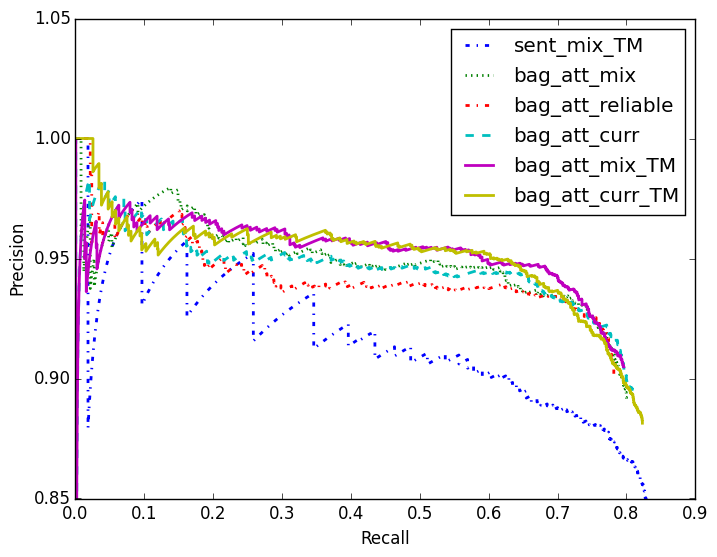
\includegraphics[width=0.45\linewidth]{figures/bag_att_exp_overall.png}
\label{fig: bag_att_luo}
}
\subfigure[Average Aggregation]{
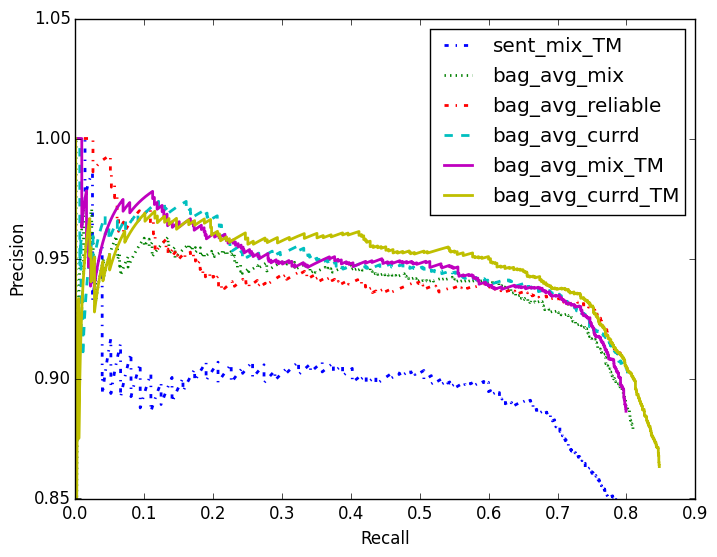
\includegraphics[width=0.45\linewidth]{figures/bag_avg_exp_overall.png}
\label{fig: bag_avg_luo}
}
\caption{Bag Level Results on Time RE}
\label{fig: results_on_luo}
\end{figure*}

\paragraph{Bag Level Attention Aggregation Models}
The results of the bag level models with attention aggregation is shown in Figure \ref{fig: bag_att_luo}. We can see that the basic bag level attention aggregation model (\emph{bag\_att\_mix}) performs very good and significantly outperforms the \emph{sent\_mix\_TM} model. Recall that the bag level model is based on the at-least-one assumption that at least one of the sentences in the sentence bag support the ($subj$, $rel$, $obj$) triple, and the \emph{sent\_mix\_TM} model do not use any assumption about the dataset. This shows that prior knowledge of the data quality plays an important role in the situation where the dataset is noisy. In the bag level models, the curriculum learning over dataset can be conducted by using only the reliable sentences in the sentence bag, and add unreliable sentences gradually. However, we find that using only reliable subset (\emph{bag\_att\_reliable}) or using curriculum learning over dataset alone (\emph{bag\_att\_curr}) does not improve the bag level attention aggregation model. This shows that the less reliable data in the sentence bag may provide additional side information or possibly plays the role of avoiding overfitting. \todo{polish the explanation.} Also note that the at-least-one assumption does not always hold and there are also false negative and false positive problems in bag level. Therefore, we can see that using transition matrix with or without curriculum learning over the dataset (\emph{bag\_att\_curr\_TM} and \emph{bag\_att\_mix\_TM}) all improve the model performance, and the \emph{bag\_att\_curr\_TM} model performs better in the low recall region.

\paragraph{Bag Level Average Aggregation Models}
The results of the bag level models with average aggregation is shown in Figure \ref{fig: bag_avg_luo}. The ranking of each setting is similar to the attention aggregation models. One interesting thing is that our transition matrix method improves the average aggregation models more significantly than the attention aggregation models. Note that the average aggregation model actually do not have good ability of handling sentence level noise. Therefore, the unhandled sentence level noise may further propagate to the bag level, which gives the transition matrix more chance to help model the noise. Also note that the \emph{bag\_avg\_curr\_TM} model significantly outperforms the \emph{bag\_avg\_mix\_TM}, this shows that curriculum learning over dataset helps the transition matrix more when the noise is more severe.

\begin{figure}[htbp]
\begin{center}
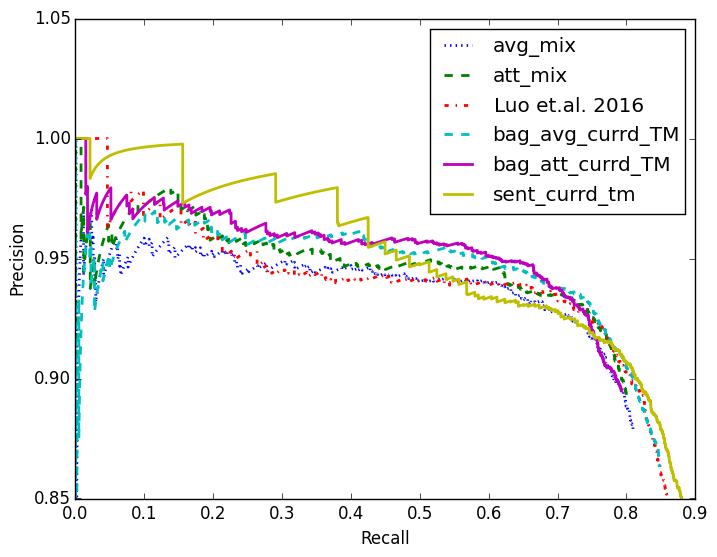
\includegraphics[width=0.9\linewidth]{figures/best_cmp_exp_overall.png}
\caption{Comparison on Time RE}
\label{fig: cmp_luo}
\end{center}
\end{figure}

\paragraph{Comparison}
\todo{polish this part}
The comparison of the best settings of each model family is shown in Figure \ref{fig: cmp_luo}. We can see that all of our models outperforms the model of \cite{luo2016temporal}. With the help of transition matrix, although the basic version of average aggregation is not as good as attention aggregation, its transition matrix version is similar to the attention aggregation. Also note that although the sentence level models trained on mixed data do not perform very good, the sentence level model can use transition matrix to model the sentence level noise and thus performs best in all these models. Recall that the transition matrix can model the noise rather than just reduce the influence of noisy sentences as in bag level models, the sentence level model actually has the ability to make use of the noisy data. This shows that sentence level noise is more important than the bag level noise in relation extraction, and modeling noise works better than just trying to reducing the influence of noise.


\begin{figure}[htbp]
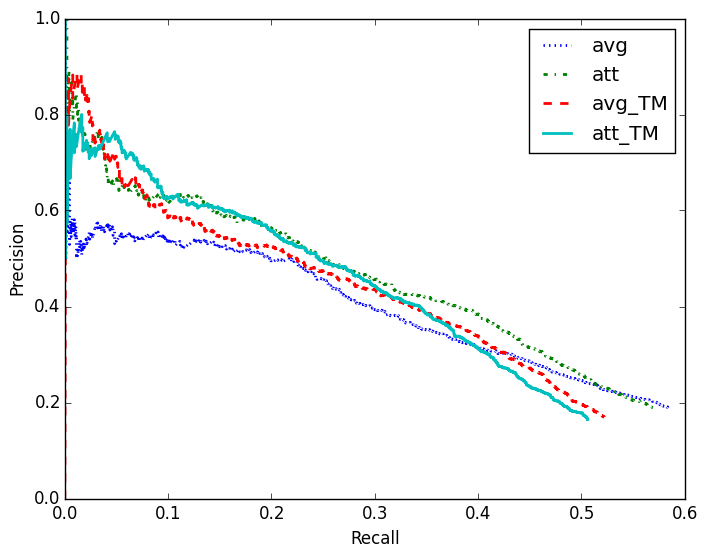
\includegraphics[width=0.9\linewidth]{figures/re_att_avg_cmp_exp.png}
\caption{Results on Dataset of Riedel et.al.}
\label{fig: Riedel_res}
\end{figure}

\subsection{Performance on Entity RE Data}
To show the generalization ability of our proposed transition matrix method, we also conduct experiments on the entity RE dataset proposed by \cite{riedel2010modeling}, which is a commonly used dataset in relation extraction. We implement the average aggregation method (\emph{avg}) and the attention aggregation method (\emph{att}) proposed by \cite{lin2016neural} as well as the corresponding transition matrix version (\emph{avg\_TM} and \emph{att\_TM}). The results are shown in Figure \ref{fig: Riedel_res}. We can see that, since the average aggregation method do not have good ability in handling sentence level noise, it performs significantly worse than the attention aggregation method. Similar to the results in time RE data, since the unhandled sentence level noise propagates to the bag level, which makes the bag level noise become more severe, the transition matrix has more chance to model the noise. Therefore, the \emph{avg\_TM} model significantly outperforms the \emph{avg} model. As for attention aggregation, this model already have good ability in reducing the impact of sentence level noise. Since the bag level noise is less important than the sentence level noise, the improvement of our transition matrix model is limited, which only improves the model on the low recall part. Note that the low recall part corresponds to high precision, which is more useful than the rest of the extraction results in practice. Therefore, our transition matrix method is also useful in this situation.

\iffalse
\begin{figure*}[htbp]
\centering
\subfigure[Overall PR Curves]{
\includegraphics[width=0.475\linewidth]{figures/reg_exp_overall.png}
\label{fig: reg_overall_pr_curve}
}
\subfigure[Small Relation PR Curves]{
\includegraphics[width=0.475\linewidth]{figures/reg_exp_small.png}
\label{fig: reg_small_rel_pr_curve}
}
\caption{Impact of Regularization Weights}
\label{fig: reg_PR_curve}
\end{figure*}
\fi
\section{Experimental Results \label{sec:evaluation}}

\begin{figure}[t!]
\begin{center}
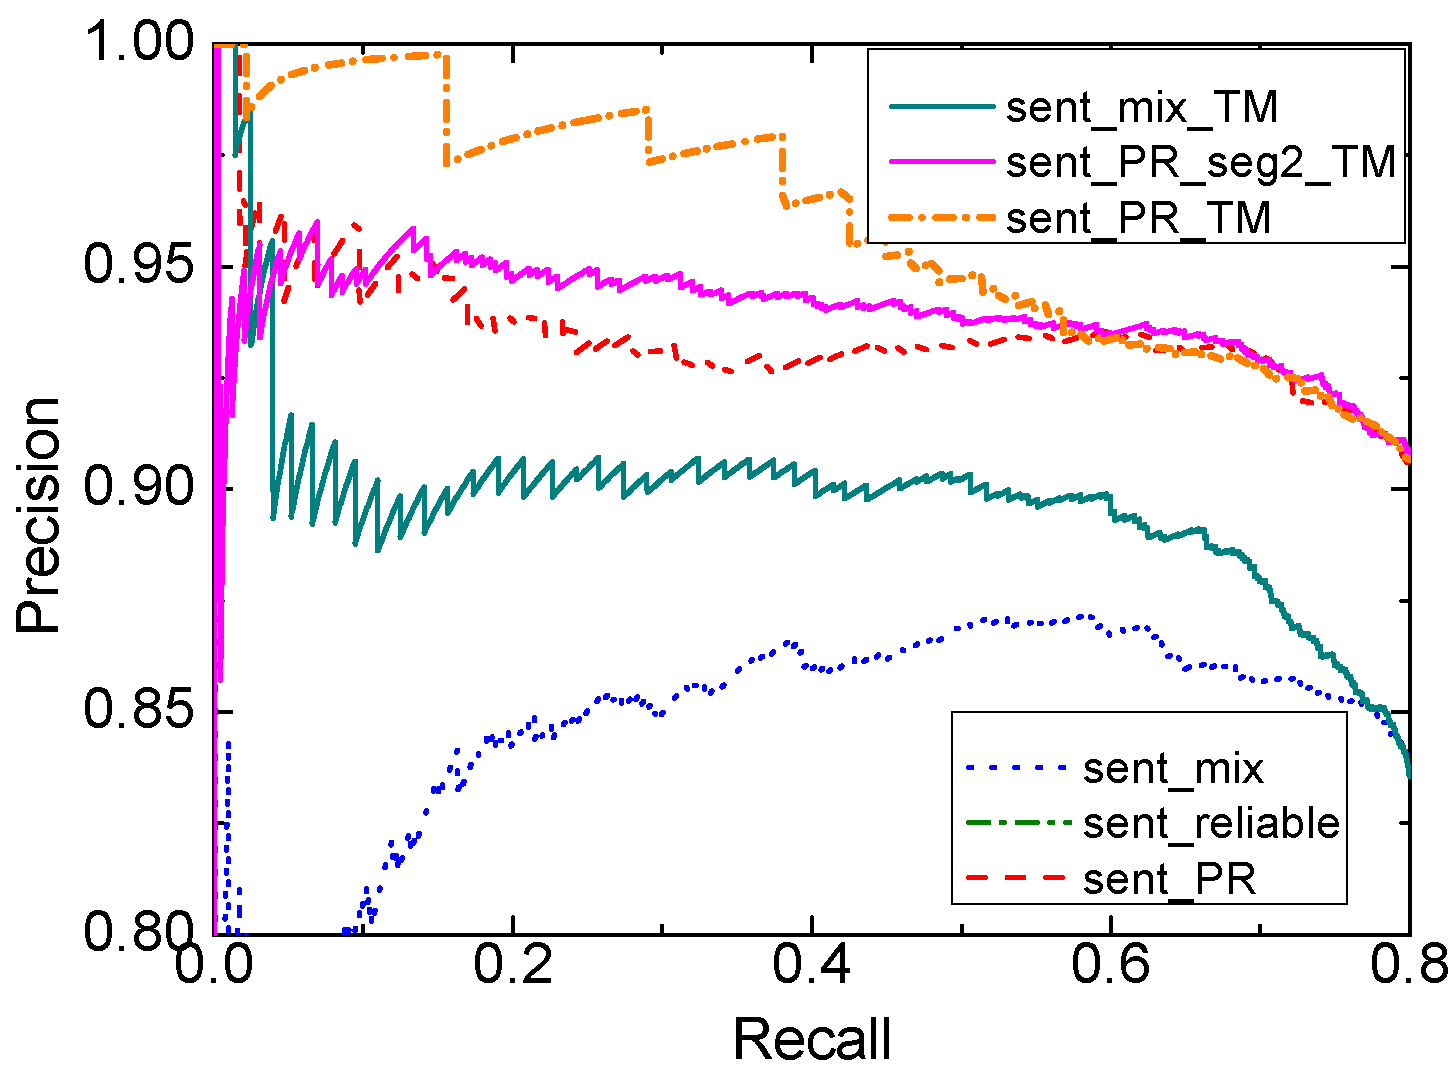
\includegraphics[width=0.48\textwidth]{figures/sent_time_exp_overall.pdf}
\caption{Sentence Level Results on \TimeRE}
\label{fig: sent_luo}
\end{center}
\end{figure}



\subsection{Performance on \TimeRE} \label{sec:results_in_TimeRE}

\paragraph{Sentence Level Models}
The results of sentence level models on \TimeRE are shown in Figure \ref{fig:
sent_luo}. We can see that mixing all subsets together (\texttt{sent\_mix})
gives the worst result. The performance of this strategey is significantly
worse than using the reliable subset only (\texttt{sent\_reliable}). This
suggests the noisy nature of the training data obtained through \DS and
properly dealing with the noise is the key for \DS to be adopted at a wider
scale. When getting help from our transition matrix during training, the
model (\texttt{sent\_mix\_TM}) significantly improves (\texttt{sent\_mix}),
delivering the same level of performance as (\texttt{sent\_reliable}) in most
cases. This suggests that our transition matrix can help to mitigate the bad influence of noisy training instances.


Let us consider the \texttt{PR} scenario where one can build a curriculum by first training on the
reliable subset and then gradually moving to the space with both reliable and less
reliable subsets. In this case, the curriculum learning based model
(\texttt{sent\_PR}) even  outperforms \emph{sent\_reliable} significantly \red{(F: does \texttt{sent\_PR} have help from other components? e.g., TM?) } \orange{No},
indicating that the curriculum learning framework not only reduces the effect
of noise, but also helps the model learns from noisy data. When applying the
transition matrix approach into this curriculum learning framework using one reliable
subset and \orange{one unreliable subset generated by mixing the two less reliable subsets, our model (\emph{sent\_PR\_seg2\_TM})
further improves \emph{sent\_PR} by  %exploring the prior knowledge about data quality and
enabling it to use transition matrix to model the noise}
%enabling the transition matrix approach to control the noise at different levels during different curriculums. }
% \todo{ZW: Have no idea of what this sentence is talking about. \textbf{I have rephrased it}.}
(\orange{I further rephrased this sentence.})
\orange{It is not surprising that when we use all three subsets separately,}
our model (\emph{sent\_PR\_TM}) significantly outperforms all
other models by a large margin\footnote{We will use all three subsets for all
\emph{\_PR} settings in the rest of the experiments.}. 

\begin{figure*}[t!]
\centering
\subfigure[Attention Aggregation]{
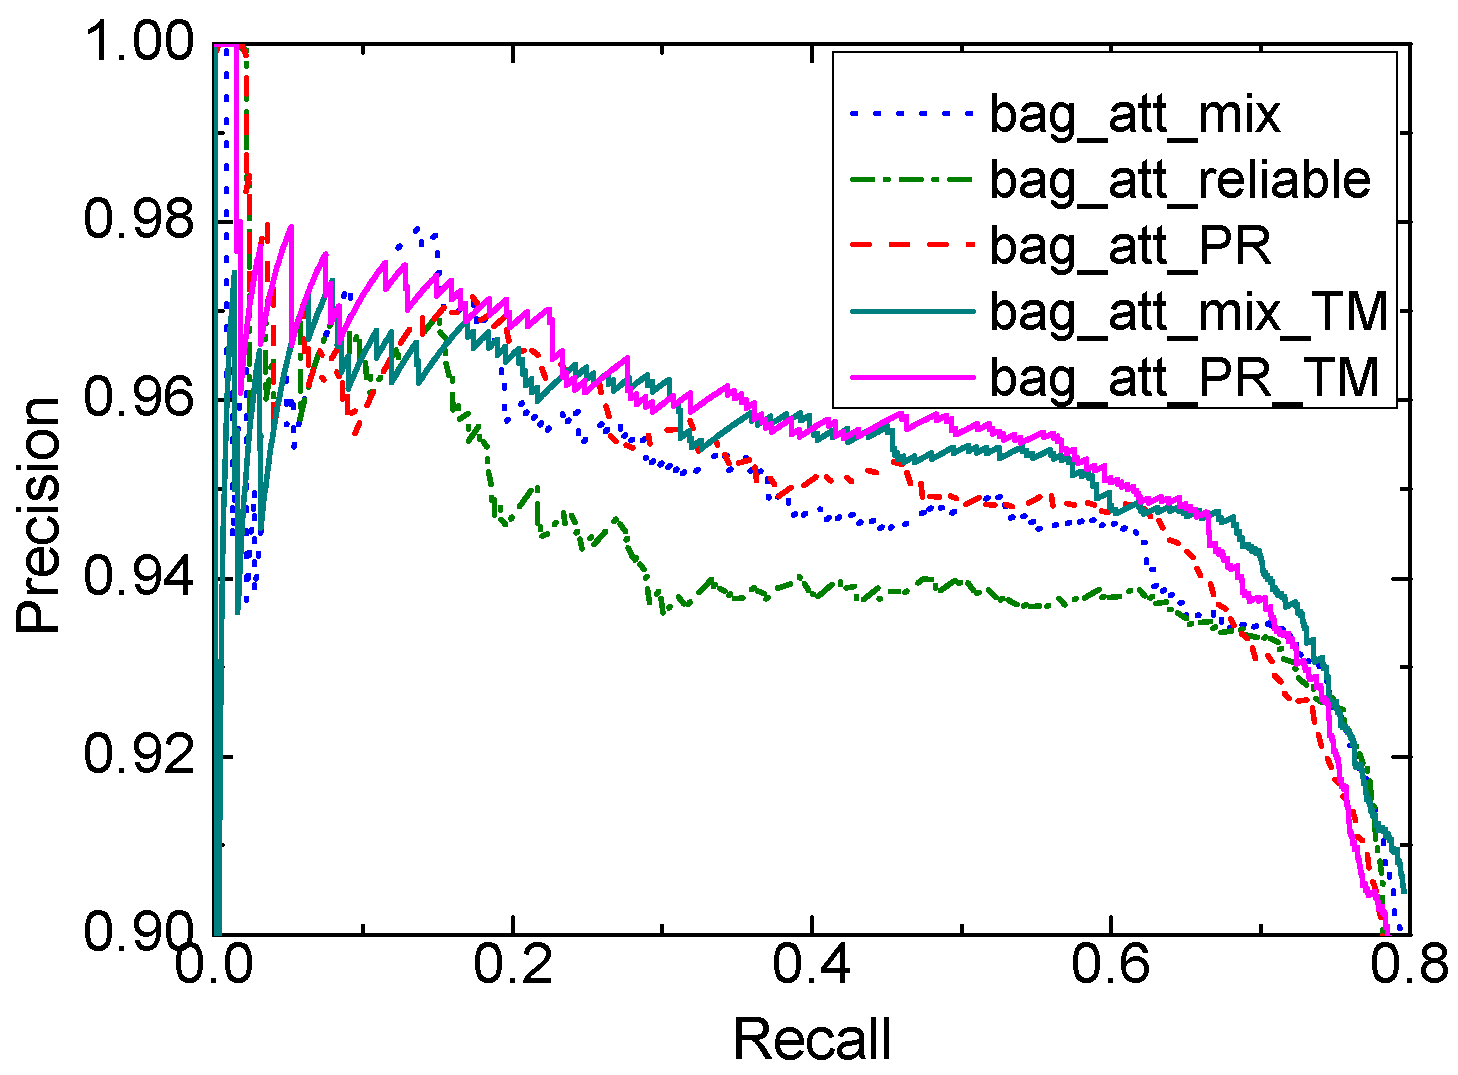
\includegraphics[width=0.48\textwidth]{figures/bag_att_exp_overall.pdf}
\label{fig: bag_att_luo}
}
\subfigure[Average Aggregation]{
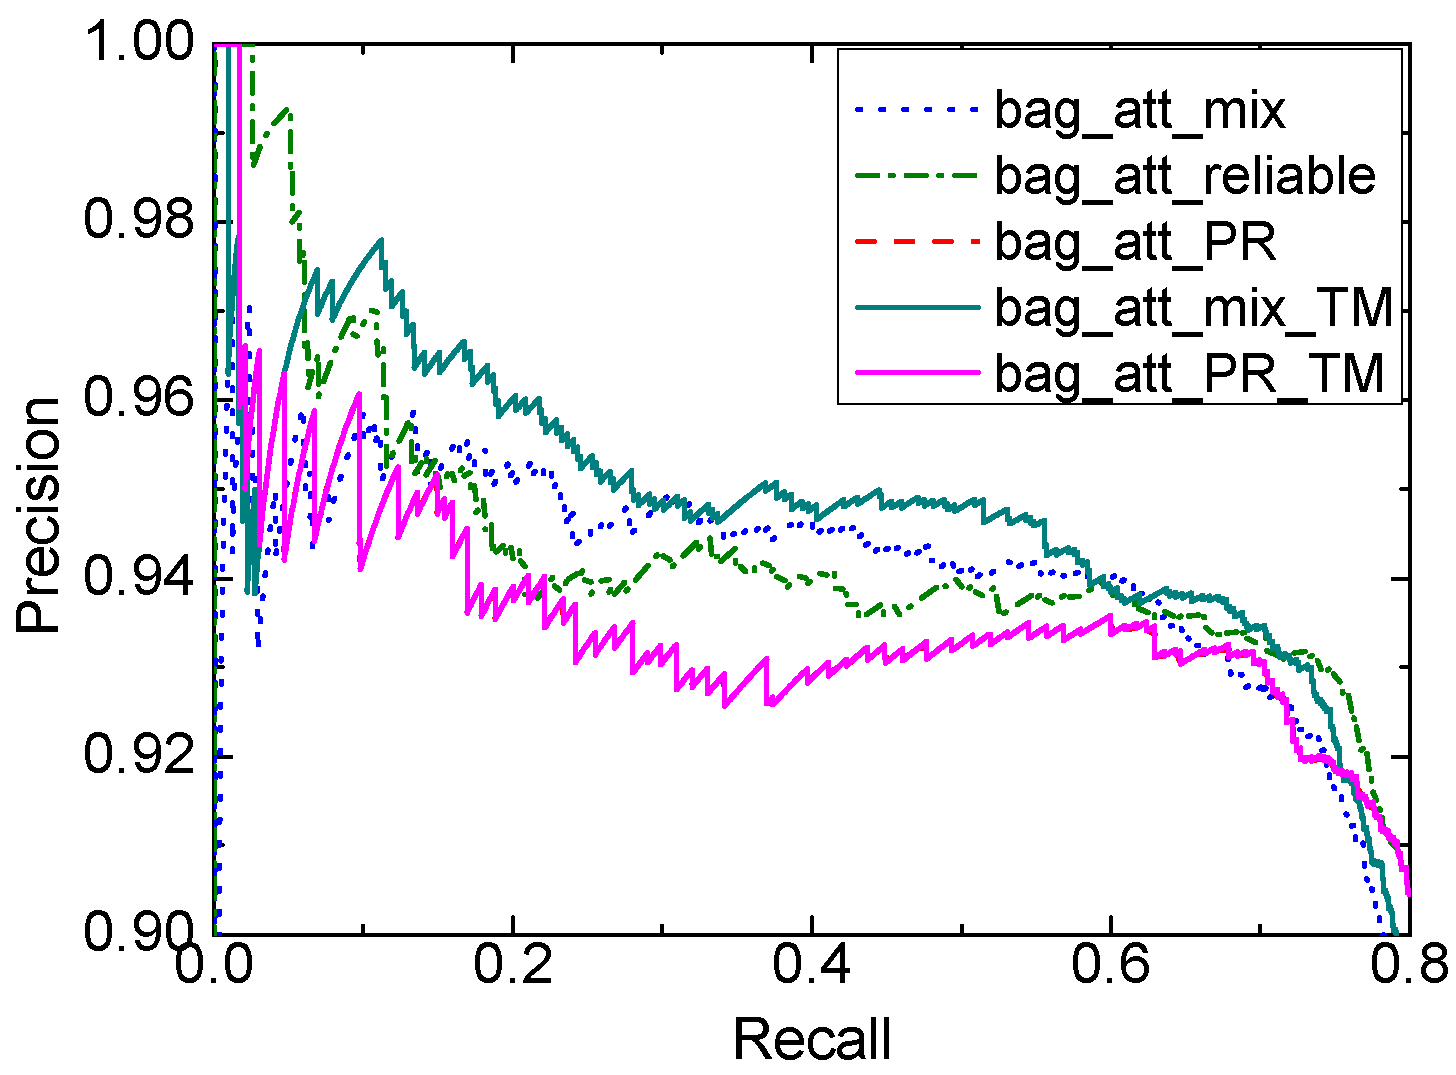
\includegraphics[width=0.48\textwidth]{figures/bag_avg_exp_overall.pdf}
\label{fig: bag_avg_luo}
}
\caption{Bag Level Results on \TimeRE}
\label{fig: results_on_luo}
\end{figure*}


\paragraph{Bag Level Models}
In this experiment, we first look at the performance of the bag level models with attention aggregation. The results are shown in Figure \ref{fig: bag_att_luo}.
Consider a comparison between the  model trained on the reliable subset only (\texttt{bag\_att\_reliable}) and the model trained on the mixed dataset (\texttt{bag\_att\_mix}).
In contrast to the sentence level cases, \texttt{bag\_att\_mix} outperforms \texttt{bag\_att\_reliable} by a large margin. This is due to the fact that \texttt{bag\_att\_mix} has taken the noise within the bag into consideration through the attention aggregation mechanism, which can be seen as a denoising step within the bag.
This may also be the reason that when we introduce either our transition matrix approach \red{(\texttt{bag\_att\_mix\_TM})}  or the curriculum of using the reliable data first (\texttt{bag\_att\_PR}) into the bad level model, the improvement compared to \texttt{bag\_att\_mix}  is not as significant as in the sentence level.
However, when we utilize our transition matrix approach to model the noise with the curriculum of using the reliable data first (\texttt{bag\_att\_PR\_TM}), the performance gets further improved. This is especially in the high precision part compared to \texttt{bag\_att\_PR}.
We also note that the bag level's \textit{at-least-one} assumption does not always hold, and there are still false negative and false positive problems. Therefore, we can see that using our transition matrix approach with or without prior knowledge of data quality, i.e., \texttt{bag\_att\_mix\_TM}  and \texttt{bag\_att\_PR\_TM}, both improve the performance, and \texttt{bag\_att\_PR\_TM} performs slightly better.

%\paragraph{Bag Level Average Aggregation Models}
The results of the bag level models with average aggregation is shown in Figure \ref{fig: bag_avg_luo}. The relative ranking of various settings is similar to those with the attention aggregation.
One of the notable differences is that both \texttt{bag\_avg\_PR} and \texttt{bag\_avg\_mix\_TM} improve \texttt{bag\_avg\_mix} with larger margins compared to that in the attention aggregation setting. The reasons may be that the average aggregation mechanism is not as good as the attention aggregation one in terms of denoising ability, which leaves more space for our transition matrix approach or curriculum learning with prior knolwdege of data quality to improve.
\orange{We can also see that \texttt{bag\_avg\_reliable} performs best in the very-low-recall region but worst in general.
This is because that it ranks highly the sentences expressing relation \emph{birth-date} and \emph{death-date} which are the simplest and the most common relations in the dataset. However, due to the less amout of data, this model performs worse in other relations and thus generates the worst results in general.}
% Therefore, this shows that training only on the reliable data leads the model to use the most common patterns with high confidence, but the less amount of data makes it performs worse in general.
%\red{why (\texttt{bag\_avg\_reliable}) performs so much better than all others in the very high precision stage ($recall<0.05$)?????????}
%\orange{Another prominent difference lies in the performance drop of \emph{bag\_avg\_PR\_TM} in the low-recall area ($recall<0.15$). With manual investigation, we find that this is caused by some high ranking of false negative data}
%However, since  denoising ability is not as good as attention aggregation, adding unreliable data gradually (\emph{bag\_avg\_currd}) improves the model performance here. We can also see that the transition matrix improves the average aggregation models more significantly than the attention aggregation models.
 %Note that due to the inferior denoising ability of average aggregation, the unhandled sentence level noise may further propagates to bag level, which gives the transition matrix more chance to help model the noise.

\begin{figure}[htbp]
\begin{center}
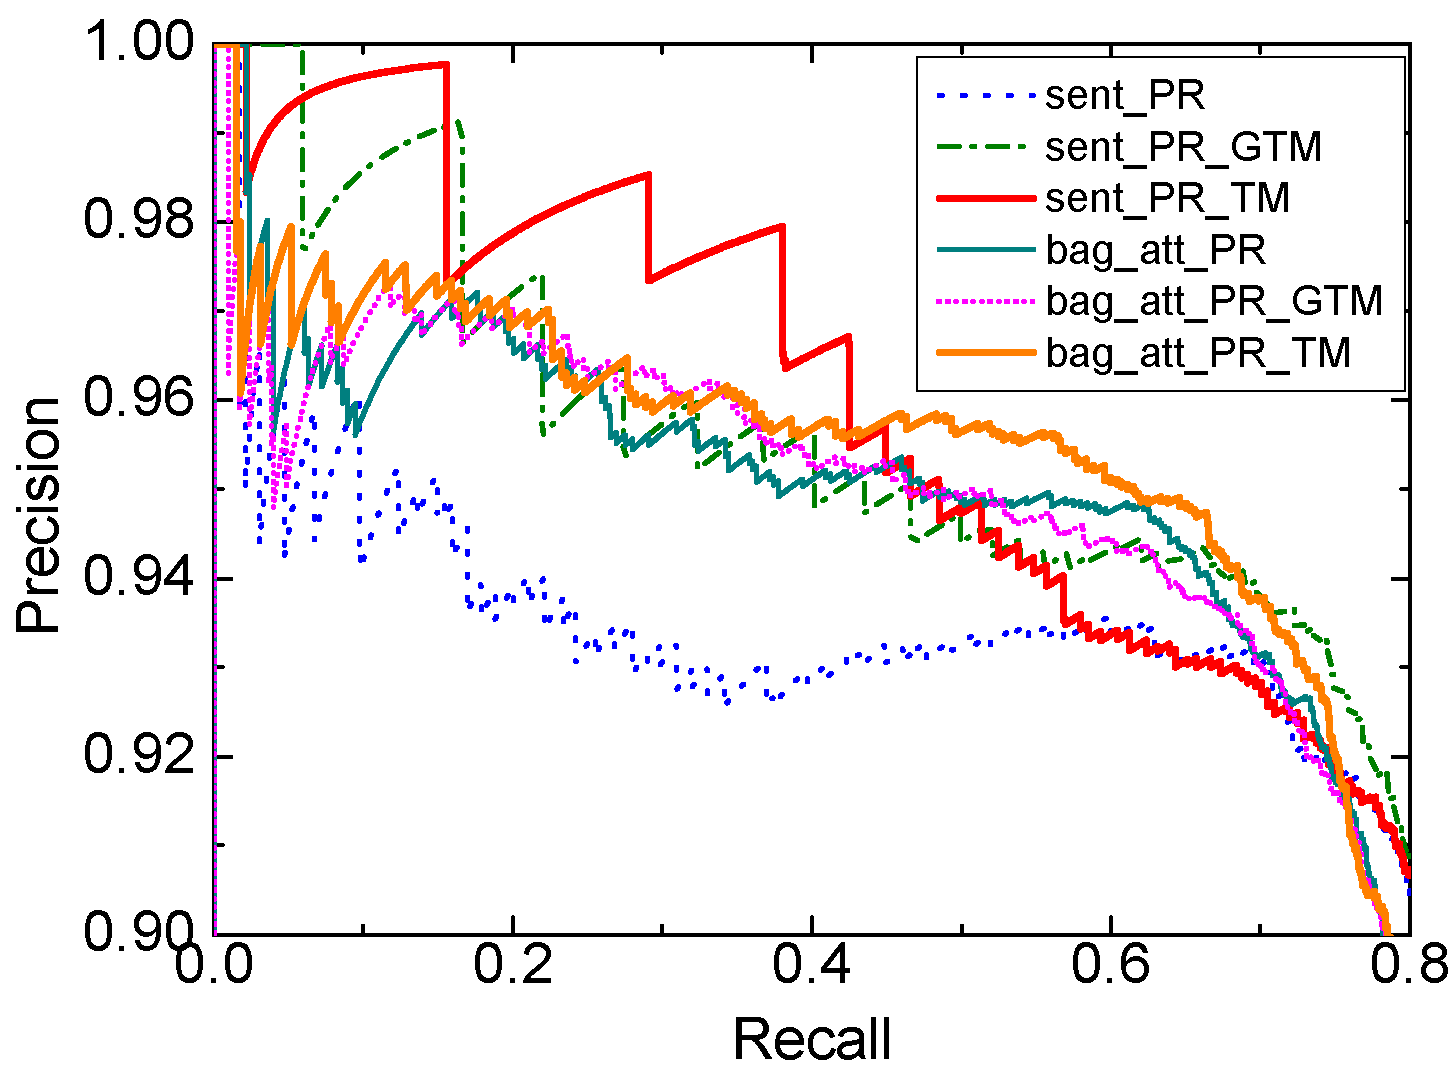
\includegraphics[width=0.48\textwidth]{figures/single_cmp_exp_overall.pdf}
\caption{Single TM vs Dynamic TM}
\label{fig: cmp_single_dynamic}
\end{center}
\end{figure}

\paragraph{Global v.s. Dynamic Transition Matrix}
We also compare our dynamic transition matrix method with the global transition matrix method.
Specifically, instead of dynamically generating a transition matrix for each datum, the global transition matrix method use a single transition matrix for all the traning data. First, we initialize an identity matrix $\mathbf{T}'\in\mathbb{R}^{k\times k}$ where $k$ is the number of relations (including \orange{\emph{no\_relation}, (unify the notation)}), then the global transition matrix is calculated with row-wise softmax:
\begin{equation}
\label{shared_mat}
T_{ij} = \frac{e^{T'_{ij}}}{\sum_{j=1}^{k}{e^{T'_{ij}}}}
\end{equation}
where $T_{ij}$ and $T'_{ij}$ are the elements in the $i^{th}$ row and $j^{th}$ column of $\mathbf{T}$ and $\mathbf{T}'$. The element values of matrix $\mathbf{T}'$ are also updated via backpropagation during training.
The results are shown in Figure \ref{fig: cmp_single_dynamic}.
We can see that using only a global transition matrix (\texttt{\_GTM}) is also beneficial and it improves both \texttt{sent\_PR} and \texttt{bag\_att\_PR}. However, since the global transition matrix only captures global noise pattern and will therefore have incorrect behavior when the data is reliable, it performs worse than our dynamic transition matrix methods (\texttt{\_TM}).

\begin{figure}[t!]
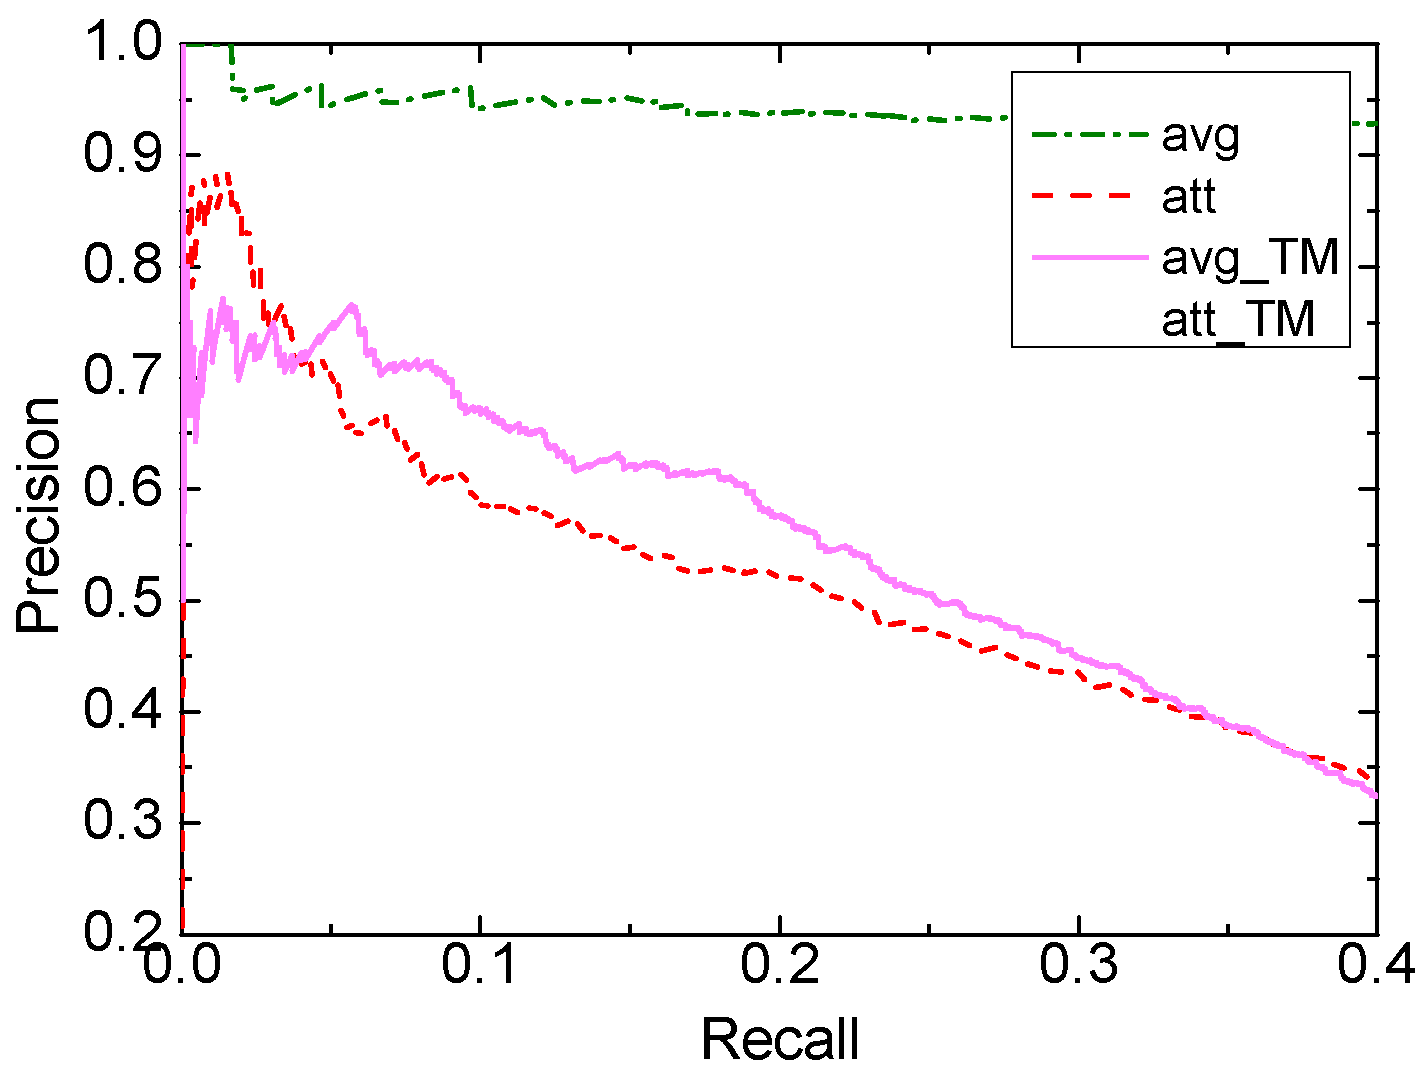
\includegraphics[width=0.48\textwidth]{figures/re_att_avg_cmp_exp.pdf}
\caption{Results on Dataset of Riedel et.al.}
\label{fig: Riedel_res}
\end{figure}

\subsection{Performance on \EntityRE}
We also conduct experiments on the \EntityRE dataset, where we can evaluate our bag level models only. 
We  implemented the average aggregation method (\texttt{avg}), and the attention aggregation method (\texttt{att}) proposed by \cite{lin2016neural} as well as their corresponding transition matrix versions (\texttt{avg\_TM} and \texttt{att\_TM}). As we can see in Figure \ref{fig: Riedel_res},  due to the inferior denoising ability of the average aggregation component, \texttt{avg} performs worst among all those models. %Similar to the trends on the TimeRE data, when
\red{what should we say about this figure????}
When we inject our transition matrix approach into both \emph{avg} and \emph{att}, the resulting two  models, both of which can  clearly outperform their basic extraction models.
%
%since the unhandled sentence level noise propagates to the bag level, which makes the bag level noise become more severe, the transition matrix has more chance to model the noise. Therefore, the \emph{avg\_TM} model clearly outperforms the \emph{avg} model.
\orange{Again, because the attention aggregation model already has good ability in reducing the impact of sentence level noise and the bag level noise is less significant than the sentence level noise, the improvement of our transition matrix model is limited, which only improves the model on the low recall part.}
%Since
%Note that the low recall part corresponds to high precision, which is more useful than the rest of the extraction results in practice. Therefore, our transition matrix method is also useful in this situation.

\subsection{Summary}
\todo{ZW: This section is incredibly complex. I suggest to have a summary section to highlight the take away messages.} 
\section{Related Work}
%\todo{add more description about DS}
%\todo{ZW: Starting by saying something like: Our work lies at the intersection of numerous areas: relation extraction, xx, xx. There is no work similar to ours, with respect to modeling the noise of training data for distant supervision and then use the knowledge of noise to improve relation extraction. We then organise the related work into different areas.}

%\paragraph{Distant Supervision in NLP} 
In addition to relation extraction, %~\cite{mintz2009distant}, 
distant supervision (\DS) is shown to be effective in generating training data for various NLP tasks, e.g., tweet sentiment
classification~\cite{go2009twitter}, tweet named entity classifying~\cite{ritter2011named}, etc.
%multi-instance learning with overlapping relations~\cite{ritter2011named}.
However, these early applications of \DS do not well address the issue of data noise.

%Due to the simplicity and the good generalization ability of distant supervision, this method has been utilized in
%many tasks. \cite{go2009twitter} builds training data for sentiment classification by using emoticons to label the
%sentiment polarity of sentences. \cite{ritter2011named} constructs entity type classification data by aligning entity
%mentions with their possible types in Freebase, \cite{duong2014can} builds POS tagging data for low-resource languages
%by translating and projecting English POS tagging results. \cite{mintz2009distant} builds relation extraction data by
%considering the sentences containing both the subject and the object of a triple in knowledge base to support the
%existence of the triple.

%\paragraph{Noise Reduction}
In relation extraction (\RE), recent works  have been proposed to reduce the influence of wrongly labeled data.
The work presented by \cite{takamatsu2012reducing} removes potential noisy sentences by identifying bad syntactic
patterns at the pre-processing stage. \cite{xu2013filling} use pseudo-relevance feedback to find
possible false negative data. 
\cite{riedel2010modeling} make the \emph{at-least-one assumption} 
%assume that at least one of the retrieved sentences containing both \emph{subj} and \emph{obj} supports the corresponding $<$\emph{subj},\emph{rel},\emph{obj}$>$ triple (i.e. \emph{at-least-one assumption})  
and 
propose to alleviate the noise problem by considering \RE  as a multi-instance classification problem.
Following this assumption, people further improves the original paradigm using probabilistic graphic models~\cite{hoffmann2011knowledge,surdeanu2012multi}, and neural network methods \cite{zeng2015distant}. 
Recently, \cite{lin2016neural} propose to use attention mechanism to reduce the noise within a sentence bag. 
%In contrast to our work in noise modeling, these approaches all aim to identify either reliable or unreliable instances to reduce
%the bad influence of noise.
Instead of characterizing the noise, these approaches only aim to alleviate the effect of noise. %reduce the bad influence of noise.
%
%Although distant supervision significantly reduces human efforts in build training data, it also introduces noise to
%the dataset. In relation extraction, \cite{takamatsu2012reducing} considers the denoising problem as a pre-processing
%problem, and removes potential noisy sentences by identifying bad syntactic patterns. \cite{riedel2010modeling}
%proposes to alleviate the noise problem by considering the relation extraction task as a multi-instance classification
%problem based on the assumption that at least one of the retrieved sentences (sentence bag) support the triple. Under
%the multi-instance classification paradigm, \cite{hoffmann2011knowledge,surdeanu2012multi} use graphic models to solve
%the problem, \cite{zeng2015distant} use piece-wise convolutional neural network (PCNN) for sentence embedding and
%\cite{lin2016neural} further proposes
%to use attention mechanism to better distinguish true positive ones from false positive ones. Instead of modeling the noise, these models actually only tries to identify the reliable sentences and reduce the influence of unreliable ones.


%\paragraph{Noise Modeling}
The \emph{at-least-one assumption} is often too strong in practice, and there are still chances that the
sentence bag may be false positive or false negative. Thus it is important to model the noise pattern 
to guide the learning procedure.
%Recent works in the area include 
\cite{ritter2013modeling} and \cite{min2013distant} try to 
employ a set of latent variables to represent the true relation. Our approach differs
from them in two aspects. 
We target  noise modeling in neutral networks while they target probabilistic graphic models. 
We further advance their models by providing the capability to model the fine-grained transition from the true relation to the observed, and 
the flexibility to combine indirect guidance.
% Third, while our model is fully differentiable, their parameters used to model the transition from true relation to observed transtion need to be set by hand or heuristics.

%\cite{ritter2013modeling,min2013distant} model the noise by adding a set of latent
%variables to the MultiR model \cite{hoffmann2011knowledge} and the MIML model \cite{surdeanu2012multi} respectively to
%represent the true relation before the observed relations.
%Our method shares similar spirit to
%\cite{ritter2013modeling} and \cite{min2013distant} in that we all generate the true relation before the observed
%relation. We differs from them in that our model is designed in the neural network framework and their models are
%designed in the probabilistic graphic model framework.
%Furthermore, our model is fully differentiable can model fine grained transition from true relation to observed relation, while their noise modeling parameters need to by set by hand or heuristics and their methods only handle false negative and false positive noise.

%the noise modeling part in our model is fully differentiable while their parameters used to model the transition from true relation to observed relation need to be set by hand or with some heuristics.


%The differences between our models are three-fold. First, our model is designed in the neural network framework and their models are designed in the probabilistic graphic model framework. Second, the noise modeling part in our model is fully differentiable while their parameters used to model the transition from true relation to observed relation need to be set by hand or with some heuristics. Third, our transition matrix model can model fine grained transition from true relation to observed relation (the sentence level noise is fine grained), while their methods only deals with false negative and false positive noise.

%This method has the problem that it also removes good sentences since the sentences containing bag patterns are not always noises.
%The noise can come from automatically constructed dataset like Tiny Images dataset \cite{torralba200880} where the images are gathered from web search engine and can also come from human labeled dataset \cite{misra2016seeing} like the MS COCO Captions dataset \cite{chen2015microsoft}.

% \paragraph{Neural Network Based Denoising} 
%Recently, 
Outside of NLP, various methods have been proposed in computer vision  to 
 model the data noise using neural networks.
\cite{sukhbaatar2014training}  utilize a global transition matrix with weight decay to transform the true label distribution to 
the observed.  %, and further propose the idea of trace regularization but use weight decay for simplicity. 
\cite{reed2014training} also use a hidden layer to represent the true label distribution but try to force it to predict both the noisy label and the input. \cite{chen2015webly,xiao2015learning} first estimate the transition matrix on a clean dataset and apply to the noisy data. 
% ~\cite{sukhbaatar2014training,reed2014training,chen2015webly,xiao2015learning,misra2016seeing}. 
Our model shares similar spirit with \cite{misra2016seeing} in that we all dynamically generate a transition matrix for each
training instance, but, instead of using Expectation-Maximization, we train our model with a novel curriculum learning training framework with trace regularization to control the behavior of noise.
In NLP, the only recent work in neural-network-based noise modeling is to use a global transition matrix only to model the noise introduced by
cross-lingual projection of training data~\cite{fang2016learning}.
 Our work advances them through generating a transition matrix dynamically for each instance, to avoid  using one single component to characterize both reliable and unreliable data. 
% This leads to significant better performance (see Section~\ref{sec:evaluation}).


% Our method is also related to the thread of work of designing denoising neural network components in computer vision.  \cite{sukhbaatar2014training} proposes to use a global transition matrix to transform the true label distribution to the observed label distribution and uses weight decay on the transition matrix during training. \cite{reed2014training} also uses a hidden layer to represent the true label distribution but try to force it to predict both the noisy label and the input. \cite{chen2015webly,xiao2015learning} first estimates the transition matrix on the clean data set and use it in the noisy data set. \cite{misra2016seeing} generates the transition matrix dynamically for each training instance.

%In natural language processing (NLP), the research on denoising with neural network is limited. \cite{fang2016learning} also uses a global transition matrix to model the noise introduced by cross-lingual projection of training data in the task of POS tagging for low-resource languages and train the basic model on the clean data first and add the transition matrix when using noisy data afterwards. Our model shares similar spirit with \cite{misra2016seeing} in that we all dynamically generate a transition matrix for each training data. However, instead of using EM, we train our model with curriculum learning and trace regularization. Furthermore, we also discuss the architecture for generating bag level transition matrix. Similar to \cite{fang2016learning}, we also have both reliable and unreliable data in one of our datasets and we also train on the reliable subset first and then add the unreliable subset. We differs from them in that we also utilize trace regularization to help the transition matrix model the noise better.

%\paragraph{First Order Temporal Fact Extraction} Since most methods designed for relation extraction can be used directly to first order temporal fact extraction, the number of researches on this subtask is limited. Recently, \cite{luo2016temporal} suggests that the multi-granular nature of time expressions can help us distinguish reliable data from unreliable ones, and they divides the the distant supervision data of first order temporal fact extraction into four subsets with different levels of reliability. They further propose to dynamically generate a weight for each instance in the training set, hoping that noisy data will be assigned lower weights and have less influence on the training procedure. They also try to randomly convert the observed relation in noisy data set to \emph{no\_relation} so that the model will be more conservative when using less reliable data. The main drawback of their model is that they only try to lower the influence of the noisy data. Therefore, much of the information hidden in the noisy data are not fully used. On the other hand, our method models the noise explicitly and it has the potential to find the real relations of noisy data. Therefore, our model can make better use of noisy data and the experiments confirms our assumption.

%\paragraph{Other Related Tasks}
%Higher order temporal fact extraction focuses on finding the valid time scope of a (subject \emph{s}, relation \emph{r}, object \emph{o}) triple. The commonly used datasets are introduced by the 2011 and 2013 temporal slot filling (TSF) shared tasks \cite{Ji2011Overview,dang2013task}. Distant supervision can also be used in this task \cite{artiles2011cuny,sil2014temporal}. Although our general idea can be possibly applied to this task, the fact that it takes triples as subjects further complicates the task, and it will be non-trivial to develop the final model for this task because the basic model need to be changed. We will leave this adaptation to future work.
%Another related task is event temporal relation identification. This task is introduced by TempEval \cite{verhagen2007semeval,pustejovsky2009semeval} and aims at extracting event-time and event-event temporal relations like \emph{before}, \emph{after}, and \emph{overlap}. Unlike previous tasks, this task mainly focuses on ordering events rather than extracting triples that take time expressions as objects, and this task is often conducted in fully supervised manner where the data set is human-labeled \cite{mani2006machine,yoshikawa2009jointly}.

\section{Conclusion}
In this paper, we investigate the noise problem inherent in  the \DS-style training data.
 We argue that the data speak for themselves by providing useful clues to reveal their noise patterns.
We thus propose a novel transition matrix based method to dynamically characterize the noise underlying such training data in a unified framework along  the original prediction objective.
One of our key innovations is to exploit a curriculum learning based training method to gradually  learn to model  the underlying noise pattern without direct guidance, and to provide the flexibility to exploit any prior knowledge of the data quality to further improve the effectiveness of the transition matrix.
We evaluate our approach in two learning settings of the distantly supervised relation extraction. The experimental results show
that the proposed method can better characterize the underlying noise and consistently outperform start-of-the-art extraction models under various scenarios.

%Currently, our noise modeling branch is relatively independent  with respect to the normal prediction branch.  which 

\section*{Acknowledgments}
We would like to thank the anonymous reviewers for their helpful
feedback. This work is supported by National High Technology R\&D Program of China (Grant
No. 2015AA015403, 2014AA015102), Natural Science Foundation of China (Grant No. 61202233,
61272344, 61370055) and the joint project with IBM Research. For any correspondence, please contact
Yansong Feng. \orange{verify this section!!}

\clearpage
\bibliography{acl2017}
\bibliographystyle{acl_natbib}

\end{document}
